% Options for packages loaded elsewhere
\PassOptionsToPackage{unicode}{hyperref}
\PassOptionsToPackage{hyphens}{url}
\PassOptionsToPackage{dvipsnames,svgnames,x11names}{xcolor}
%
\documentclass[
  12pt,
  letterpaper,
  DIV=11,
  numbers=noendperiod,
  abstract]{scrartcl}

\usepackage{amsmath,amssymb}
\usepackage{setspace}
\usepackage{iftex}
\ifPDFTeX
  \usepackage[T1]{fontenc}
  \usepackage[utf8]{inputenc}
  \usepackage{textcomp} % provide euro and other symbols
\else % if luatex or xetex
  \usepackage{unicode-math}
  \defaultfontfeatures{Scale=MatchLowercase}
  \defaultfontfeatures[\rmfamily]{Ligatures=TeX,Scale=1}
\fi
\usepackage{lmodern}
\ifPDFTeX\else  
    % xetex/luatex font selection
\fi
% Use upquote if available, for straight quotes in verbatim environments
\IfFileExists{upquote.sty}{\usepackage{upquote}}{}
\IfFileExists{microtype.sty}{% use microtype if available
  \usepackage[]{microtype}
  \UseMicrotypeSet[protrusion]{basicmath} % disable protrusion for tt fonts
}{}
\makeatletter
\@ifundefined{KOMAClassName}{% if non-KOMA class
  \IfFileExists{parskip.sty}{%
    \usepackage{parskip}
  }{% else
    \setlength{\parindent}{0pt}
    \setlength{\parskip}{6pt plus 2pt minus 1pt}}
}{% if KOMA class
  \KOMAoptions{parskip=half}}
\makeatother
\usepackage{xcolor}
\setlength{\emergencystretch}{3em} % prevent overfull lines
\setcounter{secnumdepth}{5}
% Make \paragraph and \subparagraph free-standing
\makeatletter
\ifx\paragraph\undefined\else
  \let\oldparagraph\paragraph
  \renewcommand{\paragraph}{
    \@ifstar
      \xxxParagraphStar
      \xxxParagraphNoStar
  }
  \newcommand{\xxxParagraphStar}[1]{\oldparagraph*{#1}\mbox{}}
  \newcommand{\xxxParagraphNoStar}[1]{\oldparagraph{#1}\mbox{}}
\fi
\ifx\subparagraph\undefined\else
  \let\oldsubparagraph\subparagraph
  \renewcommand{\subparagraph}{
    \@ifstar
      \xxxSubParagraphStar
      \xxxSubParagraphNoStar
  }
  \newcommand{\xxxSubParagraphStar}[1]{\oldsubparagraph*{#1}\mbox{}}
  \newcommand{\xxxSubParagraphNoStar}[1]{\oldsubparagraph{#1}\mbox{}}
\fi
\makeatother

\usepackage{color}
\usepackage{fancyvrb}
\newcommand{\VerbBar}{|}
\newcommand{\VERB}{\Verb[commandchars=\\\{\}]}
\DefineVerbatimEnvironment{Highlighting}{Verbatim}{commandchars=\\\{\}}
% Add ',fontsize=\small' for more characters per line
\usepackage{framed}
\definecolor{shadecolor}{RGB}{241,243,245}
\newenvironment{Shaded}{\begin{snugshade}}{\end{snugshade}}
\newcommand{\AlertTok}[1]{\textcolor[rgb]{0.68,0.00,0.00}{#1}}
\newcommand{\AnnotationTok}[1]{\textcolor[rgb]{0.37,0.37,0.37}{#1}}
\newcommand{\AttributeTok}[1]{\textcolor[rgb]{0.40,0.45,0.13}{#1}}
\newcommand{\BaseNTok}[1]{\textcolor[rgb]{0.68,0.00,0.00}{#1}}
\newcommand{\BuiltInTok}[1]{\textcolor[rgb]{0.00,0.23,0.31}{#1}}
\newcommand{\CharTok}[1]{\textcolor[rgb]{0.13,0.47,0.30}{#1}}
\newcommand{\CommentTok}[1]{\textcolor[rgb]{0.37,0.37,0.37}{#1}}
\newcommand{\CommentVarTok}[1]{\textcolor[rgb]{0.37,0.37,0.37}{\textit{#1}}}
\newcommand{\ConstantTok}[1]{\textcolor[rgb]{0.56,0.35,0.01}{#1}}
\newcommand{\ControlFlowTok}[1]{\textcolor[rgb]{0.00,0.23,0.31}{\textbf{#1}}}
\newcommand{\DataTypeTok}[1]{\textcolor[rgb]{0.68,0.00,0.00}{#1}}
\newcommand{\DecValTok}[1]{\textcolor[rgb]{0.68,0.00,0.00}{#1}}
\newcommand{\DocumentationTok}[1]{\textcolor[rgb]{0.37,0.37,0.37}{\textit{#1}}}
\newcommand{\ErrorTok}[1]{\textcolor[rgb]{0.68,0.00,0.00}{#1}}
\newcommand{\ExtensionTok}[1]{\textcolor[rgb]{0.00,0.23,0.31}{#1}}
\newcommand{\FloatTok}[1]{\textcolor[rgb]{0.68,0.00,0.00}{#1}}
\newcommand{\FunctionTok}[1]{\textcolor[rgb]{0.28,0.35,0.67}{#1}}
\newcommand{\ImportTok}[1]{\textcolor[rgb]{0.00,0.46,0.62}{#1}}
\newcommand{\InformationTok}[1]{\textcolor[rgb]{0.37,0.37,0.37}{#1}}
\newcommand{\KeywordTok}[1]{\textcolor[rgb]{0.00,0.23,0.31}{\textbf{#1}}}
\newcommand{\NormalTok}[1]{\textcolor[rgb]{0.00,0.23,0.31}{#1}}
\newcommand{\OperatorTok}[1]{\textcolor[rgb]{0.37,0.37,0.37}{#1}}
\newcommand{\OtherTok}[1]{\textcolor[rgb]{0.00,0.23,0.31}{#1}}
\newcommand{\PreprocessorTok}[1]{\textcolor[rgb]{0.68,0.00,0.00}{#1}}
\newcommand{\RegionMarkerTok}[1]{\textcolor[rgb]{0.00,0.23,0.31}{#1}}
\newcommand{\SpecialCharTok}[1]{\textcolor[rgb]{0.37,0.37,0.37}{#1}}
\newcommand{\SpecialStringTok}[1]{\textcolor[rgb]{0.13,0.47,0.30}{#1}}
\newcommand{\StringTok}[1]{\textcolor[rgb]{0.13,0.47,0.30}{#1}}
\newcommand{\VariableTok}[1]{\textcolor[rgb]{0.07,0.07,0.07}{#1}}
\newcommand{\VerbatimStringTok}[1]{\textcolor[rgb]{0.13,0.47,0.30}{#1}}
\newcommand{\WarningTok}[1]{\textcolor[rgb]{0.37,0.37,0.37}{\textit{#1}}}

\providecommand{\tightlist}{%
  \setlength{\itemsep}{0pt}\setlength{\parskip}{0pt}}\usepackage{longtable,booktabs,array}
\usepackage{calc} % for calculating minipage widths
% Correct order of tables after \paragraph or \subparagraph
\usepackage{etoolbox}
\makeatletter
\patchcmd\longtable{\par}{\if@noskipsec\mbox{}\fi\par}{}{}
\makeatother
% Allow footnotes in longtable head/foot
\IfFileExists{footnotehyper.sty}{\usepackage{footnotehyper}}{\usepackage{footnote}}
\makesavenoteenv{longtable}
\usepackage{graphicx}
\makeatletter
\newsavebox\pandoc@box
\newcommand*\pandocbounded[1]{% scales image to fit in text height/width
  \sbox\pandoc@box{#1}%
  \Gscale@div\@tempa{\textheight}{\dimexpr\ht\pandoc@box+\dp\pandoc@box\relax}%
  \Gscale@div\@tempb{\linewidth}{\wd\pandoc@box}%
  \ifdim\@tempb\p@<\@tempa\p@\let\@tempa\@tempb\fi% select the smaller of both
  \ifdim\@tempa\p@<\p@\scalebox{\@tempa}{\usebox\pandoc@box}%
  \else\usebox{\pandoc@box}%
  \fi%
}
% Set default figure placement to htbp
\def\fps@figure{htbp}
\makeatother
% definitions for citeproc citations
\NewDocumentCommand\citeproctext{}{}
\NewDocumentCommand\citeproc{mm}{%
  \begingroup\def\citeproctext{#2}\cite{#1}\endgroup}
\makeatletter
 % allow citations to break across lines
 \let\@cite@ofmt\@firstofone
 % avoid brackets around text for \cite:
 \def\@biblabel#1{}
 \def\@cite#1#2{{#1\if@tempswa , #2\fi}}
\makeatother
\newlength{\cslhangindent}
\setlength{\cslhangindent}{1.5em}
\newlength{\csllabelwidth}
\setlength{\csllabelwidth}{3em}
\newenvironment{CSLReferences}[2] % #1 hanging-indent, #2 entry-spacing
 {\begin{list}{}{%
  \setlength{\itemindent}{0pt}
  \setlength{\leftmargin}{0pt}
  \setlength{\parsep}{0pt}
  % turn on hanging indent if param 1 is 1
  \ifodd #1
   \setlength{\leftmargin}{\cslhangindent}
   \setlength{\itemindent}{-1\cslhangindent}
  \fi
  % set entry spacing
  \setlength{\itemsep}{#2\baselineskip}}}
 {\end{list}}
\usepackage{calc}
\newcommand{\CSLBlock}[1]{\hfill\break\parbox[t]{\linewidth}{\strut\ignorespaces#1\strut}}
\newcommand{\CSLLeftMargin}[1]{\parbox[t]{\csllabelwidth}{\strut#1\strut}}
\newcommand{\CSLRightInline}[1]{\parbox[t]{\linewidth - \csllabelwidth}{\strut#1\strut}}
\newcommand{\CSLIndent}[1]{\hspace{\cslhangindent}#1}

% load packages
\usepackage{geometry}
\usepackage{xcolor}
\usepackage{eso-pic}
\usepackage{fancyhdr}
\usepackage{sectsty}
\usepackage{fontspec}
\usepackage{titlesec}

%% Set page size with a wider right margin
\geometry{a4paper, total={170mm,257mm}, left=20mm, top=20mm, bottom=20mm, right=50mm}

%% Let's define some colours
\definecolor{light}{HTML}{E6E6E7}
\definecolor{highlight}{HTML}{00883A}
\definecolor{dark}{HTML}{345442}

%% Let's add the border on the right hand side 
\AddToShipoutPicture{% 
    \AtPageLowerLeft{% 
        \put(\LenToUnit{\dimexpr\paperwidth-3cm},0){% 
            \color{light}\rule{3cm}{\LenToUnit\paperheight}%
          }%
     }%
     % logo
    \AtPageLowerLeft{% start the bar at the bottom right of the page
        \put(\LenToUnit{\dimexpr\paperwidth-2.25cm},27.2cm){% move it to the top right
            \color{light}
\includegraphics[width=2cm]{_extensions/nrennie/PrettyPDF/logo.png}
          }%
     }%
}

%% Style the page number
\fancypagestyle{mystyle}{
  \fancyhf{}
  \renewcommand\headrulewidth{0pt}
  \fancyfoot[R]{\thepage}
  \fancyfootoffset{3.5cm}
}
\setlength{\footskip}{20pt}

%% style the chapter/section fonts
\chapterfont{\color{dark}\fontsize{20}{16.8}\selectfont}
\sectionfont{\color{dark}\fontsize{20}{16.8}\selectfont}
\subsectionfont{\color{dark}\fontsize{14}{16.8}\selectfont}
\titleformat{\subsection}
  {\sffamily\Large\bfseries}{\thesection}{1em}{}[{\titlerule[0.8pt]}]
  
% left align title
\makeatletter
\renewcommand{\maketitle}{\bgroup\setlength{\parindent}{0pt}
\begin{flushleft}
  {\sffamily\huge\textbf{\MakeUppercase{\@title}}} \vspace{0.3cm} \newline
  {\Large {\@subtitle}} \newline
  \@author
\end{flushleft}\egroup
}
\makeatother

%% Use some custom fonts
\setsansfont{Ubuntu}[
    Path=_extensions/nrennie/PrettyPDF/Ubuntu/,
    Scale=0.9,
    Extension = .ttf,
    UprightFont=*-Regular,
    BoldFont=*-Bold,
    ItalicFont=*-Italic,
    ]

\setmainfont{Ubuntu}[
    Path=_extensions/nrennie/PrettyPDF/Ubuntu/,
    Scale=0.9,
    Extension = .ttf,
    UprightFont=*-Regular,
    BoldFont=*-Bold,
    ItalicFont=*-Italic,
    ]
\usepackage{fvextra}
\DefineVerbatimEnvironment{Highlighting}{Verbatim}{
    commandchars=\\\{\},
    breaklines, breaknonspaceingroup, breakanywhere
}
\KOMAoption{captions}{tableheading}
\makeatletter
\@ifpackageloaded{caption}{}{\usepackage{caption}}
\AtBeginDocument{%
\ifdefined\contentsname
  \renewcommand*\contentsname{Table of contents}
\else
  \newcommand\contentsname{Table of contents}
\fi
\ifdefined\listfigurename
  \renewcommand*\listfigurename{List of Figures}
\else
  \newcommand\listfigurename{List of Figures}
\fi
\ifdefined\listtablename
  \renewcommand*\listtablename{List of Tables}
\else
  \newcommand\listtablename{List of Tables}
\fi
\ifdefined\figurename
  \renewcommand*\figurename{Figure}
\else
  \newcommand\figurename{Figure}
\fi
\ifdefined\tablename
  \renewcommand*\tablename{Table}
\else
  \newcommand\tablename{Table}
\fi
}
\@ifpackageloaded{float}{}{\usepackage{float}}
\floatstyle{ruled}
\@ifundefined{c@chapter}{\newfloat{codelisting}{h}{lop}}{\newfloat{codelisting}{h}{lop}[chapter]}
\floatname{codelisting}{Listing}
\newcommand*\listoflistings{\listof{codelisting}{List of Listings}}
\makeatother
\makeatletter
\makeatother
\makeatletter
\@ifpackageloaded{caption}{}{\usepackage{caption}}
\@ifpackageloaded{subcaption}{}{\usepackage{subcaption}}
\makeatother
\makeatletter
\@ifpackageloaded{tcolorbox}{}{\usepackage[skins,breakable]{tcolorbox}}
\makeatother
\makeatletter
\@ifundefined{shadecolor}{\definecolor{shadecolor}{rgb}{.97, .97, .97}}{}
\makeatother
\makeatletter
\@ifundefined{codebgcolor}{\definecolor{codebgcolor}{named}{light}}{}
\makeatother
\makeatletter
\ifdefined\Shaded\renewenvironment{Shaded}{\begin{tcolorbox}[frame hidden, breakable, colback={codebgcolor}, sharp corners, enhanced, boxrule=0pt]}{\end{tcolorbox}}\fi
\makeatother

\usepackage{bookmark}

\IfFileExists{xurl.sty}{\usepackage{xurl}}{} % add URL line breaks if available
\urlstyle{same} % disable monospaced font for URLs
\hypersetup{
  pdftitle={Exploring Bot Detection on Reddit},
  pdfauthor={Matteo Mazzarelli},
  colorlinks=true,
  linkcolor={highlight},
  filecolor={Maroon},
  citecolor={Blue},
  urlcolor={highlight},
  pdfcreator={LaTeX via pandoc}}


\title{Exploring Bot Detection on Reddit}
\usepackage{etoolbox}
\makeatletter
\providecommand{\subtitle}[1]{% add subtitle to \maketitle
  \apptocmd{\@title}{\par {\large #1 \par}}{}{}
}
\makeatother
\subtitle{Computational Social Science WS2024/25}
\author{Matteo Mazzarelli}
\date{March 24, 2025}

\begin{document}
\maketitle
\begin{abstract}
In the digital age, automated accounts or bots on social media platforms
like Reddit pose a significant threat to online discourse. This paper
investigates the efficacy of basic heuristic methods for detecting bot
influence on Reddit discussions. Employing the Reddit API, we collected
data from five high-traffic subreddits and applied a heuristic-based bot
detection method utilizing meta-metrics such as account age, karma,
posting frequency, content repetitiveness, and em-dash presence.
Exploratory analysis using machine learning classifiers provided
preliminary validation of the heuristic approach in identifying bot-like
accounts based on these meta-metrics. However, keyword frequency and
sentiment analysis, aided by Large Language Models, revealed no
statistically significant content-based differences between accounts
flagged as potential bots and non-flagged accounts, suggesting bots are
increasingly capable of mimicking human language at a surface level.
While heuristics effectively flagged accounts exhibiting bot-like
behavior, they proved insufficient for content-based bot identification
without further nuanced analysis. This study highlights the limitations
of relying solely on meta-metrics and basic content analysis for bot
detection, underscoring the necessity for future research to incorporate
human-validated content labeling and advanced machine learning
techniques capable of discerning subtle linguistic cues in bot-generated
text. The development of content-aware bot detection methods is crucial
for maintaining the integrity of online discussions on platforms like
Reddit.
\end{abstract}

\pagestyle{mystyle}


\setstretch{1}
\newpage

\tableofcontents

\newpage

\section{Introduction}\label{introduction}

The pervasive presence of automated accounts, or bots, on social media
platforms has become a significant concern in the digital age. These
bots, designed to mimic human users, can manipulate online discussions,
disseminate misinformation, and potentially influence public opinion,
thus posing a threat to the integrity of online
communities\textsuperscript{{[}\citeproc{ref-botdetectionreddit}{1}{]}}.
Reddit, a platform structured around user-created communities known as
subreddits, is not immune to this issue. In fact, the platform's history
even includes the deliberate use of fake accounts to simulate activity
and attract genuine users, highlighting a long-standing awareness of the
impact of artificial
engagement\textsuperscript{{[}\citeproc{ref-redditbotproblem}{2}{]}}. As
bot technology becomes increasingly sophisticated, driven by
advancements in artificial intelligence, the need for effective
detection methods is more critical than
ever\textsuperscript{{[}\citeproc{ref-botdetectionreddit}{1}{]}}. This
paper investigates the detection of bots on Reddit, exploring the
efficacy of heuristic-based methods and the potential of large language
models (LLMs) to aid in this complex task.

The central research question guiding this study is: \textbf{Can basic
heuristic methods effectively identify bot influence on Reddit
discussions?}

This question is relevant for several reasons. Firstly, understanding
the extent of bot influence on Reddit is crucial for maintaining the
platform's credibility as a space for authentic discussion and
information sharing. Secondly, the development of effective bot
detection methods is essential to mitigate the potential negative
impacts of bots, such as the spread of misinformation and the
manipulation of public opinion. This research adds to the existing
knowledge on identifying social media bots by specifically examining
Reddit, a platform with unique characteristics that may require tailored
detection strategies. Previous research has explored various methods for
bot detection on social media, often focusing on platforms like
Twitter\textsuperscript{{[}\citeproc{ref-redditbotwatch}{3},\citeproc{ref-multibotdetector}{4}{]}}.
However, Reddit's community-driven structure and specific user behaviors
necessitate a dedicated investigation into bot detection within this
environment. This paper aims to contribute to this research gap by
evaluating the effectiveness of simple heuristic methods, readily
implementable and interpretable, in identifying bot influence on Reddit.
Furthermore, while exploring the potential of leveraging advanced LLMs
for keyword extraction and sentiment summarization to gain insights into
bot-driven narratives, it acknowledges that truly leveraging LLMs for
content-based bot detection would require a different approach, such as
labeling comment content for supervised learning. By combining
traditional heuristic methods with explorations into AI techniques, this
study aims to provide insights into both the practical applicability of
simpler approaches and the potential directions for more sophisticated
AI-driven solutions in the ongoing effort to detect and understand bot
activity on Reddit.

\section{Previous Predictive
Research}\label{previous-predictive-research}

The detection of bots on social media platforms is an area of increasing
scholarly attention, driven by the growing recognition of bots'
potential to manipulate online discourse and influence public
opinion\textsuperscript{{[}\citeproc{ref-multibotdetector}{4}{]}}.
Existing research in this field has primarily focused on platforms like
Twitter, examining a range of features and methodologies for identifying
automated
accounts\textsuperscript{{[}\citeproc{ref-redditbotwatch}{3}{]}}.

One prominent area of research involves the use of machine learning for
bot detection. Studies have explored various algorithms, including
tree-based classifiers like Random
Forests\textsuperscript{{[}\citeproc{ref-breiman2001random}{5}{]}} and
Decision
Trees\textsuperscript{{[}\citeproc{ref-breiman1984classification}{6}{]}},
as well as more complex deep learning models such as Long Short-Term
Memory (LSTM)
networks\textsuperscript{{[}\citeproc{ref-multibotdetector}{4},\citeproc{ref-evalsocialbotmodels}{7},\citeproc{ref-hochreiter1997long}{8}{]}}.
These approaches typically rely on a combination of features,
encompassing user metadata, activity patterns, and content
characteristics, to classify accounts as either bots or humans. For
instance, ensemble
methods\textsuperscript{{[}\citeproc{ref-dietterich2000ensemble}{9}{]}},
which combine multiple classifiers, have demonstrated promising results
in multi-platform bot detection, achieving notable accuracy
rates\textsuperscript{{[}\citeproc{ref-multibotdetector}{4},\citeproc{ref-multibotdetector}{4}{]}}.

Another significant research direction focuses on anomaly detection
techniques, which aim to identify accounts exhibiting behaviors that
deviate significantly from typical human user
patterns\textsuperscript{{[}\citeproc{ref-anomalycloudflare}{10}--\citeproc{ref-chandola2009anomaly}{12}{]}}.
These unsupervised learning methods are particularly valuable for
detecting novel bot behaviors that may not be captured by supervised
learning models trained on pre-labeled data. Histogram-Based Outlier
Scoring
(HBOS)\textsuperscript{{[}\citeproc{ref-goldstein2012histogram}{13}{]}}
is one such algorithm that has been applied to scalable anomaly
detection in large datasets, demonstrating its potential for identifying
unusual activity patterns indicative of bot
behavior\textsuperscript{{[}\citeproc{ref-anomalycloudflare}{10}{]}}.

While a substantial body of research exists on bot detection in social
media, fewer studies have specifically focused on
Reddit\textsuperscript{{[}\citeproc{ref-botdetectionreddit}{1},\citeproc{ref-redditbotnetwork}{14},\citeproc{ref-mlredditbots}{15}{]}}.
Reddit's unique structure, characterized by topic-specific subreddits
and community-driven moderation, presents both distinct challenges and
opportunities for bot detection. Research focusing on Reddit has begun
to explore platform-specific features, such as user interaction networks
within subreddits, to identify bot
activity\textsuperscript{{[}\citeproc{ref-redditbotnetwork}{14}{]}}.
Furthermore, studies have investigated the role of bots in specific
contexts on Reddit, such as political discussions and the dissemination
of
misinformation\textsuperscript{{[}\citeproc{ref-botdetectionreddit}{1},\citeproc{ref-multibotdetector}{4}{]}}.

Publicly available datasets play a crucial role in advancing research in
this field. While datasets specifically labeled for Reddit bot detection
are less abundant compared to those for Twitter, resources like the
Pushshift Reddit
Dataset\textsuperscript{{[}\citeproc{ref-pushshiftredditdataset}{16}{]}}
and the Reddit Comments
Dataset\textsuperscript{{[}\citeproc{ref-redditcommentsdataset}{17}{]}}
offer valuable opportunities for researchers to collect and analyze
Reddit-specific
data\textsuperscript{{[}\citeproc{ref-multibotdetector}{4},\citeproc{ref-pushshiftredditdataset}{16},\citeproc{ref-redditcommentsdataset}{17}{]}}.
These datasets, while not always labeled for bot activity, provide rich
information on user comments, posts, and metadata that can be used to
develop and evaluate bot detection methods.

It is important to note that while existing research has explored
content-based features to some extent, truly leveraging the textual
content of comments for bot detection often requires labeled data where
human experts or advanced LLMs have categorized comments as originating
from bots or humans. This type of labeled data, specifically for Reddit
comment content, remains a relatively underexplored area, highlighting a
gap that future research could address.

In summary, previous predictive research on bot detection has
established a solid foundation of methodologies and features, primarily
focused on platforms like Twitter. However, the unique characteristics
of Reddit necessitate further investigation into tailored detection
strategies for this platform. This paper builds upon this existing
research by exploring the applicability of basic heuristic methods for
Reddit bot detection and by investigating the potential of LLMs for
keyword extraction and sentiment summarization as exploratory tools. It
also acknowledges the crucial next step of incorporating content-based
analysis, which would ideally involve labeled comment data, to move
beyond meta-metrics and enhance bot detection accuracy on Reddit. By
focusing on Reddit-specific data and combining heuristic approaches with
AI explorations, this study aims to contribute to the growing body of
knowledge on social media bot detection and address the specific
challenges posed by bot activity on Reddit.

\section{Data, Methods, and Models}\label{data-methods-and-models}

\subsection{Data}\label{data}

The data for this study was collected using the Reddit API via the
Python Reddit API Wrapper
(PRAW)\textsuperscript{{[}\citeproc{ref-praw2024}{18}{]}}. The final
data collection period spanned March 21 and 22, 2025. The unit of
analysis is individual Reddit comments, as well as the users posting
them.

\textbf{Subreddit Selection:} Subreddits were selected based on their
high subscriber counts and relevance to topics frequently targeted by
bots, such as politics and news. To ensure a reproducible and systematic
subreddit selection, keywords were generated using Google
Gemini\textsuperscript{{[}\citeproc{ref-googleai2023gemini}{19}{]}}, a
large language model API. The prompt provided to Gemini requested
keywords associated with controversial topics likely to attract bot
activity. (See the Appendix for the prompt and code used for keyword
generation). Based on these keywords and subscriber counts, a scoring
system was developed to rank subreddits by their potential vulnerability
to bot influence. (See the Appendix for the scoring system and selected
subreddits). The top 10 subreddits according to this scoring system were
initially considered. For in-depth analysis and LLM querying, 5
subreddits with high bot influence scores were chosen: r/worldnews,
r/news, r/politics, r/science, and r/technology, as they are
representative of discussion topics that are likely to be targeted by
bots.

\textbf{Data Collection Procedure:} For each selected subreddit, the
Reddit API was used to collect posts and associated comments. The data
collected included:

\begin{itemize}
\tightlist
\item
  \textbf{Posts:} Post titles, post IDs, author usernames, subreddit
  names, submission types, timestamps of creation (UTC), and post text
  (selftext).
\item
  \textbf{Comments:} Comment IDs, author usernames, comment bodies,
  timestamps of creation (UTC), comment scores, comment levels (for
  nested comments), parent comment IDs, and post IDs.
\item
  \textbf{User Data:} For each comment author, publicly available user
  data such as account age (in days) and combined karma score (comment
  and link karma) were collected. Furthermore, to establish user
  behavior, the 10 most recent comments at the time of collection made
  by each of the users present in the comments dataset were sourced
  through the API. This allowed us to compute content similarity and
  posting frequency.
\end{itemize}

To manage data volume and processing time, as well as to respect API
limitations, the number of posts and comments collected were limited.
For each subreddit, the 50 hottest posts were fetched, and for each
post, a maximum of 2000 comments were collected recursively,
encompassing all comment levels. This hierarchical approach aimed to
capture a representative sample of discussions within each subreddit
while managing computational resources.

\subsection{Measurement}\label{measurement}

\textbf{Bot Identification (Heuristics):} A heuristic-based bot
detection method was implemented, flagging accounts as potential bots if
they exhibited a combination of the following characteristics:

\begin{itemize}
\tightlist
\item
  \textbf{Young Account Age:} Accounts less than a week old were
  considered potentially bot-like.
\item
  \textbf{Unusual Karma:} Accounts with unusually low or high karma
  scores relative to their activity were flagged. Thresholds for
  ``unusual'' were empirically determined based on the data
  distribution.
\item
  \textbf{High Posting Frequency:} Accounts with exceptionally high
  posting frequency, commenting multiple times within unusually short
  time intervals, were considered suspicious.
\item
  \textbf{Speed of Commenting:} Accounts commenting on posts (or
  replying to parent comments made by different users) in an
  unlikely-to-be-human quick fashion are flagged as likely to be bots.
\item
  \textbf{Repetitive Content:} Accounts frequently posting or commenting
  with highly similar or identical text were flagged for repetitive
  content. Cosine similarity of comment text was used to quantify
  content repetition.
\item
  \textbf{Em-dash Presence:} The presence of em-dashes (---) in comments
  was considered as a potential indicator of AI-generated content, as
  some AI models tend to overuse this punctuation mark, which is not
  usually present in human writing due to its difficulty in being typed
  on a normal
  keyboard\textsuperscript{{[}\citeproc{ref-redditbotdetector}{20}--\citeproc{ref-nightwateremdash}{22}{]}}.
\end{itemize}

These heuristics were chosen based on common bot characteristics
identified in previous research and community discussions on
Reddit\textsuperscript{{[}\citeproc{ref-redditbotslearnusetalents}{23}--\citeproc{ref-botproblem7daystodie}{25}{]}},
and incorporating recent observations about AI-generated text
markers\textsuperscript{{[}\citeproc{ref-redditbotdetector}{20}--\citeproc{ref-nightwateremdash}{22}{]}}.
A ``Bot Score'' was calculated for each account based on the number of
heuristics triggered. Accounts exceeding a certain threshold on the
``Bot Score'' were classified as ``possible bots'' or ``very likely
bots'' allowing for varying degrees of bot likelihood assessment. It is
important to note that these heuristics primarily rely on meta-metrics
and basic content features, and do not deeply analyze the semantic
content of the comments themselves.

\textbf{Polarization:} A basic measure of polarization was added using
sentiment analysis of comment content. The VADER (Valence Aware
Dictionary and sEntiment
Reasoner)\textsuperscript{{[}\citeproc{ref-hutto2014vader}{26}{]}}
sentiment analysis tool was employed to calculate compound sentiment
scores for comments. Average sentiment scores were compared between
comments from accounts flagged as potential bots and those from
non-flagged accounts to identify potential differences in sentiment
polarity, which could indicate bot-driven polarization.

\subsection{Models}\label{models}

\textbf{Heuristic Bot Detection Model:} The core model employed in this
study is a heuristic-based bot detection system. This model does not
rely on traditional machine learning classification but instead uses a
set of predefined rules (heuristics) based on observable account
characteristics to identify potential bots. The specific heuristics and
their implementation are detailed in the ``Measurement'' section above
and in the provided code.

\textbf{Large Language Model (LLM) for Keyword Extraction and Sentiment
Summarization:} Google Gemini, a state-of-the-art LLM, configured for
deterministic output (temperature parameter set to 0), was utilized to
extract keywords and generate sentiment summaries for comments within
each of the 5 subreddits. The prompt provided to Gemini requested:

\begin{enumerate}
\def\labelenumi{\arabic{enumi}.}
\tightlist
\item
  \textbf{Keyword Extraction:} Identification of 20 unique keywords
  capturing the essence of each subreddit's discussions, based
  exclusively on a large sample of comments.
\item
  \textbf{Sentiment Summary:} A brief summary of the overall sentiment
  expressed in the comments, indicating whether the tone was positive,
  negative, or neutral.
\end{enumerate}

The LLM's output was then parsed to extract the keyword list and
sentiment summary for each subreddit. Word clouds were generated from
the extracted keywords to visually represent the dominant themes within
each subreddit's discussions. It's important to note that while LLMs are
used here for analysis, they are not directly integrated into the
heuristic bot detection model itself, and their role is primarily
exploratory in this study, as it is not possible to produce a fully
deterministic result by querying a LLM.

\textbf{Evaluation of Bot Detection Effectiveness:} The effectiveness of
the heuristic-based bot detection method was evaluated both
qualitatively and quantitatively.

\begin{itemize}
\item
  \textbf{Qualitative Evaluation:} A manual review of accounts flagged
  as potential bots was conducted to assess the face validity of the
  heuristics and examine the characteristics of flagged accounts.
  Subreddit-specific word clouds generated from LLM keyword extraction
  were analyzed to understand the thematic focus of discussions and
  potentially identify bot-driven narratives. Sentiment summaries
  provided by the LLM were evaluated for their coherence and consistency
  with the overall tone of subreddit discussions.
\item
  \textbf{Quantitative Evaluation (Exploratory):} To explore the
  potential for quantitative evaluation, simple classification models
  (Random
  Forest\textsuperscript{{[}\citeproc{ref-breiman2001random}{5}{]}},
  SVMs\textsuperscript{{[}\citeproc{ref-cortes1995support}{27}{]}},
  Neural
  Network\textsuperscript{{[}\citeproc{ref-lecun2015deep}{28}{]}}, all
  left untuned) were trained using features derived from the heuristic
  analysis (Bot Score, account age, karma, posting frequency, content
  repetitiveness, em-dash presence, etc.). The performance of these
  models was assessed using standard classification metrics. This
  quantitative evaluation was exploratory, given the lack of a true
  ``ground truth'' dataset for bot identification in this study and the
  limitation of relying solely on meta-metrics and basic content
  features without labeled content data. It aimed to provide a
  preliminary indication of the heuristic-based approach's predictive
  capability and guide future research directions involving more
  rigorous machine learning evaluation that incorporates content-based
  features from labeled data.
\end{itemize}

\subsection{Reproducibility}\label{reproducibility}

To ensure the (partial, given the nature of the usage of LLMs at various
points) reproducibility of this research, all code used for data
collection, analysis, and model implementation is provided in the
supplementary materials. The code includes:

\begin{itemize}
\tightlist
\item
  \textbf{Data Collection Scripts:} Python scripts using PRAW to access
  the Reddit API and collect posts, comments, and user data.
\item
  \textbf{Heuristic Bot Detection Implementation:} Code implementing the
  heuristic-based bot detection rules and Bot Score calculation,
  including em-dash detection.
\item
  \textbf{LLM Querying and Keyword Extraction:} Python code using the
  Google Gemini API to query the LLM for keyword extraction and
  sentiment summaries.
\item
  \textbf{Data Analysis and Visualization Scripts:} R and Python scripts
  for data processing, statistical analysis, sentiment analysis, word
  cloud generation, and exploratory machine learning model training and
  evaluation.
\end{itemize}

The code is designed to be as self-contained and well-commented as
possible to facilitate replication by other researchers. The stochastic
elements of LLM output are minimized by setting the temperature
parameter to 0.

\section{Empirical Results}\label{empirical-results}

\subsection{Descriptive Summary of Heuristic
Criteria}\label{descriptive-summary-of-heuristic-criteria}

The heuristic-based method, designed to flag accounts based on
pre-defined meta-metric criteria, identified a specific subset of Reddit
accounts. It is essential to understand that this section describes the
output of the heuristic flagging process itself, and does not present
independently validated findings about actual bot characteristics. The
following keyword and sentiment analyses, presented next, similarly do
not provide such independent validation. Therefore, this section is best
understood as a brief, factual report on the direct output of the
heuristic flagging process, rather than a conclusive analysis of bot
characteristics. The limitations of this approach are further discussed
in the conclusion.

\subsection{Cross-Subreddit Content Similarity and Narrative
Amplification}\label{cross-subreddit-content-similarity-and-narrative-amplification}

To understand the relationships between the top subreddits in terms of
content, and to explore potential narrative amplification, a
cross-subreddit content similarity analysis was conducted.
Figure~\ref{fig-cross} displays a heatmap visualizing the cosine
similarity of TF-IDF
vectors\textsuperscript{{[}\citeproc{ref-salton1988term}{29}{]}}
generated from the combined text of comments within each of the top 5
subreddits.

As shown in Figure~\ref{fig-cross}, the heatmap reveals moderate content
similarity between certain subreddits. r/news and r/worldnews exhibit
one of the highest content similarities (0.81), which is expected given
their overlapping topical focus on current events. r/politics also shows
relatively high similarity with r/news (0.80) and r/worldnews (0.72),
indicating thematic connections between political discussions and news
reporting. r/technology and r/science show lower similarity with the
news and politics subreddits, reflecting their distinct subject matter.
r/science and r/technology exhibit moderate similarity to each other
(0.63). This suggests a thematic clustering where news and politics
subreddits are more closely related in content, while technology and
science form a separate, though somewhat related, cluster. Bots
operating across these subreddits might exploit these thematic
connections to amplify narratives across related communities.

\begin{figure}

\centering{

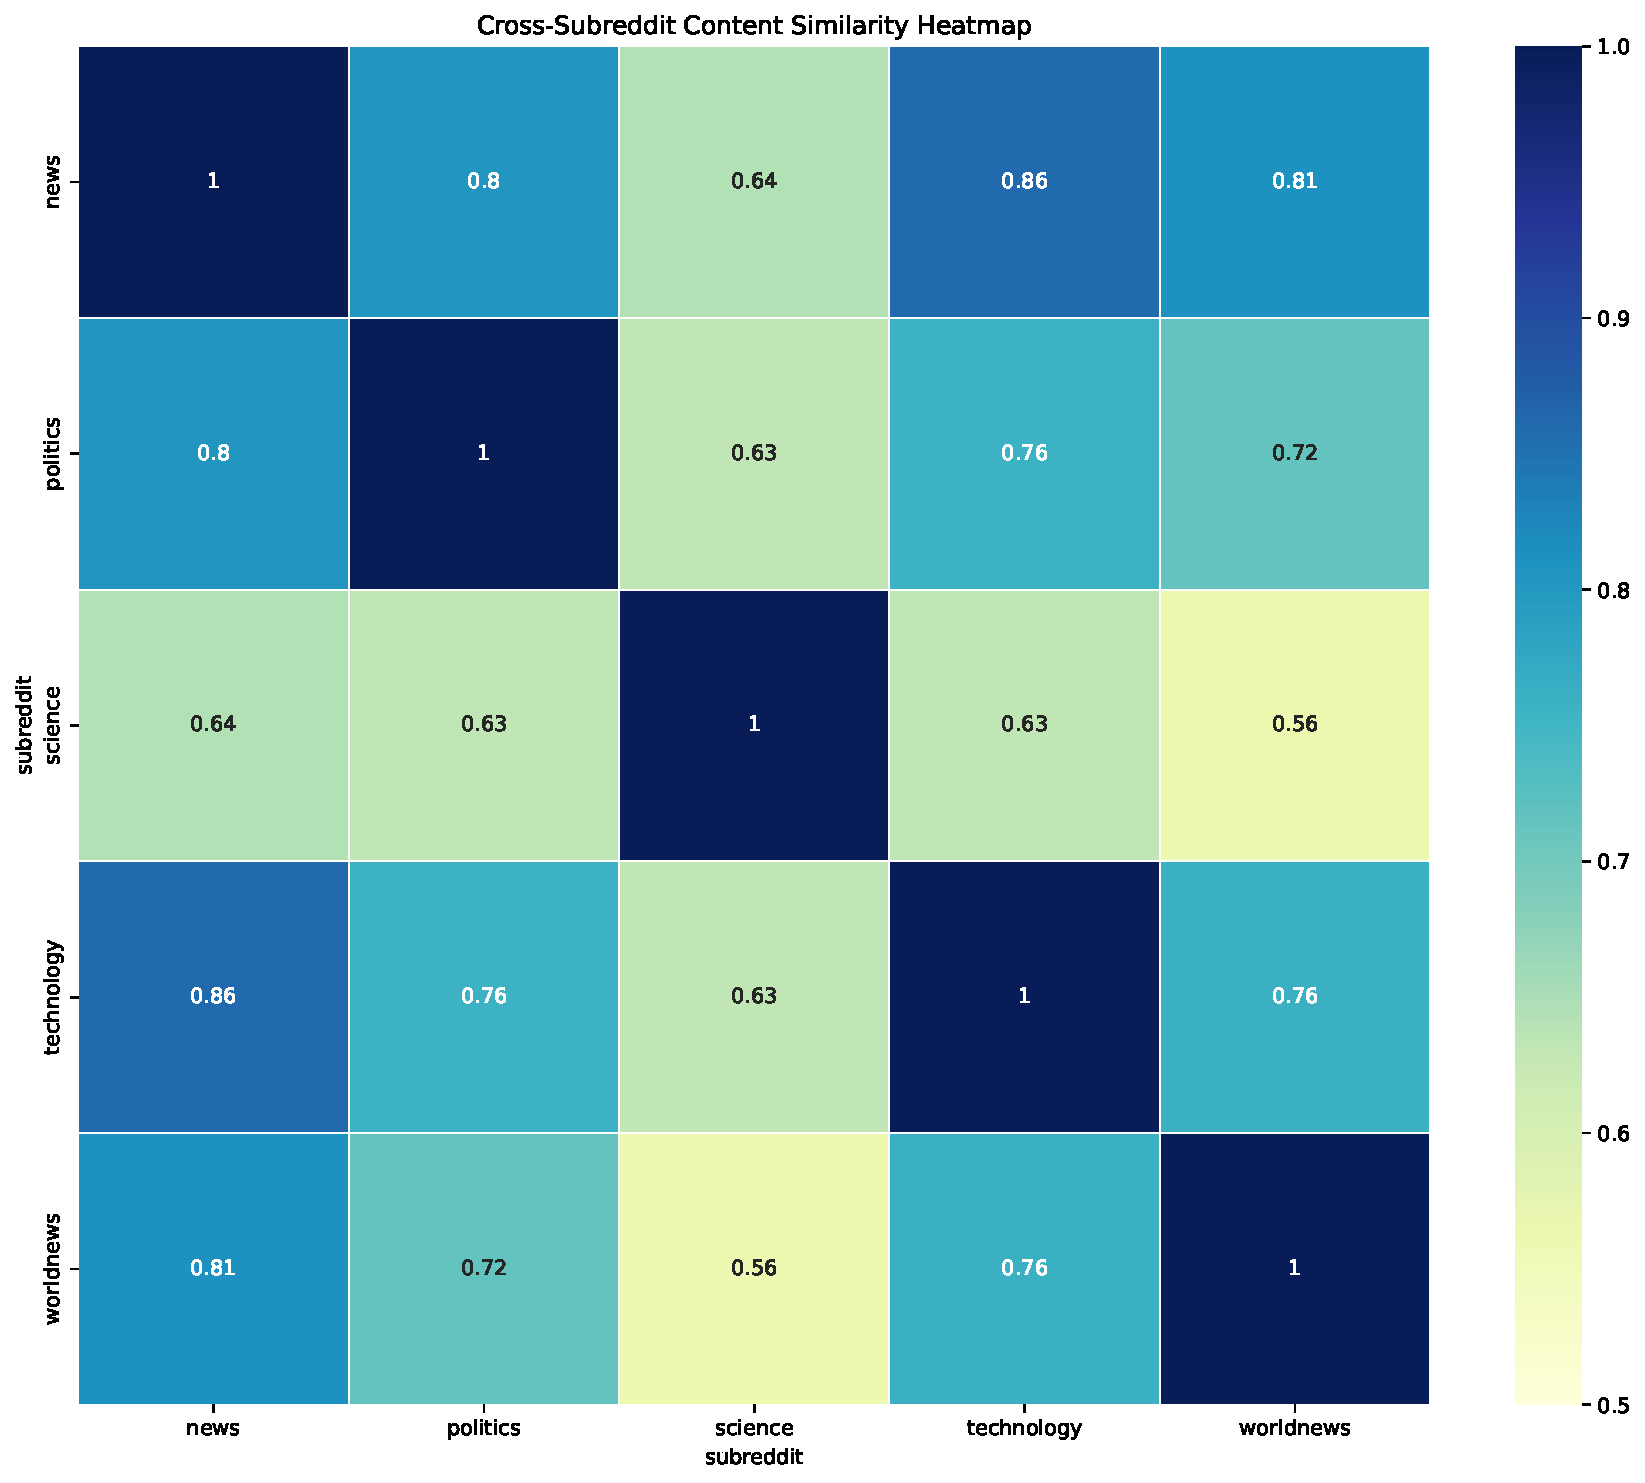
\includegraphics[width=0.85\linewidth,height=\textheight,keepaspectratio]{detecting_bots_on_reddit_code_files/figure-pdf/cell-28-output-1.pdf}

}

\caption{\label{fig-cross}Cross-Subreddit Content Similarity Heatmap:
the heatmap visualizes the cosine similarity of TF-IDF vectors between
the top 5 subreddits, with darker colors indicating higher similarity
and lighter colors indicating lower similarity.}

\end{figure}%

Analysis of keyword frequencies and sentiment scores provided further
insights into potential narrative amplification and polarization
associated with flagged accounts.

\begin{itemize}
\tightlist
\item
  \textbf{Keyword Analysis:} Figure~\ref{fig-polwc} shows the word cloud
  generated by Google Gemini for the r/politics subreddit as an example.
  Keywords like ``government,'' ``election,'' ``Democrats,'' and
  ``Trump'' are prominently featured, reflecting the politically charged
  nature of discussions in this subreddit. Keywords generated by Google
  Gemini for subreddits like r/politics and r/worldnews, which are known
  to be prone to bot activity, were frequently observed in comments from
  flagged accounts. These keywords often related to politically charged
  topics, conspiracy theories, and divisive narratives. While flagged
  accounts exhibited a numerically higher frequency of these
  bot-influence keywords compared to non-flagged accounts, the
  difference was not statistically significant in this analysis. This
  suggests that, based solely on keyword frequency, bots and humans in
  these subreddits may not differ substantially in their topical focus
  when analyzed with simple methods.
\end{itemize}

\begin{figure}

\centering{

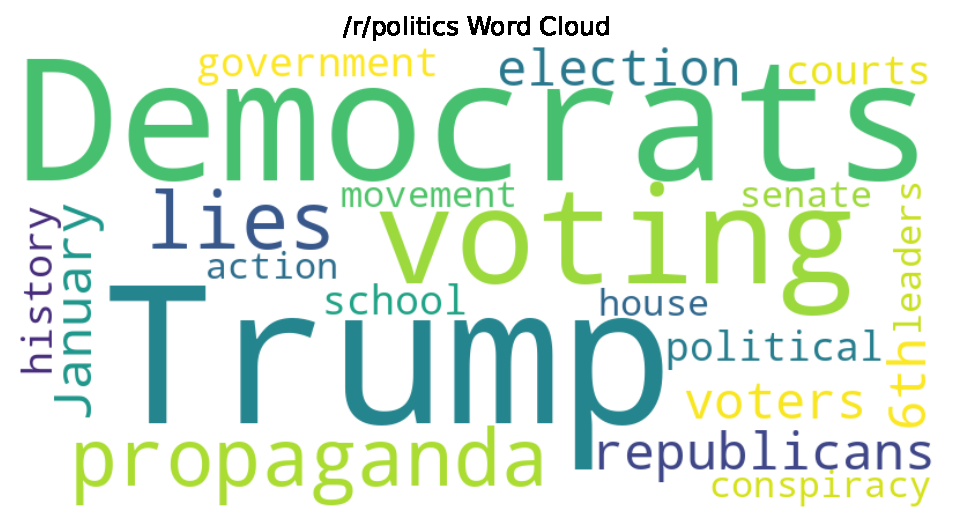
\includegraphics[width=0.85\linewidth,height=\textheight,keepaspectratio]{detecting_bots_on_reddit_code_files/figure-pdf/cell-29-output-2.pdf}

}

\caption{\label{fig-polwc}Word Cloud for /r/politics as generated by the
Gemini LLM based on a large sample of comments from the subreddit.}

\end{figure}%

\begin{itemize}
\tightlist
\item
  \textbf{Sentiment Analysis:} Sentiment analysis using VADER revealed
  subtle differences in the average sentiment polarity of comments from
  flagged and non-flagged accounts. However, similar to keyword
  analysis, this difference in average sentiment was not statistically
  significant. This indicates that, based on sentiment scores alone,
  distinguishing between bot and human comments remains challenging with
  basic sentiment analysis tools, suggesting bots may be capable of
  mimicking human sentiment expression to some extent, especially in an
  age where state of the art human-like text generation has an extremely
  low barrier of access.
\end{itemize}

The lack of statistically significant differences in keyword frequencies
and sentiment scores between flagged and non-flagged accounts suggests
that, when relying solely on these metrics, bots may be increasingly
adept at mimicking human language patterns, at least at a surface level
of topic and sentiment. This underscores the limitation of relying
solely on simple content analysis or meta-metrics for bot detection and
points to the need for more nuanced approaches that consider the deeper
semantic and contextual aspects of comment content, potentially through
human or advanced LLM-based content labeling.

\subsection{Exploratory Quantitative Evaluation of Bot
Detection}\label{exploratory-quantitative-evaluation-of-bot-detection}

Exploratory quantitative evaluation using simple machine learning
classifiers provided a preliminary assessment of the heuristic-based bot
detection approach.

\begin{itemize}
\item
  \textbf{Classification Model Performance:} Random Forest, SVM, and
  Neural Network classifiers were trained to distinguish between flagged
  and non-flagged accounts using the heuristic-derived features.
\item
  \textbf{Feature Importance:} Feature importance analysis from the best
  performing model, the Random Forest model, indicated that posting
  frequency and content repetitiveness were the most influential
  features in distinguishing between flagged and non-flagged accounts.
  This is shown in Figure~\ref{fig-importance}. Account age, karma
  score, and em-dash presence also contributed to the model's predictive
  capability, albeit to a lesser extent. This reinforces the idea that
  behavioral patterns, captured by meta-metrics like posting frequency
  and content repetition, are more indicative of bot activity than
  simple content analysis of keywords or sentiment in this heuristic
  approach.
\end{itemize}

\begin{figure}

\centering{

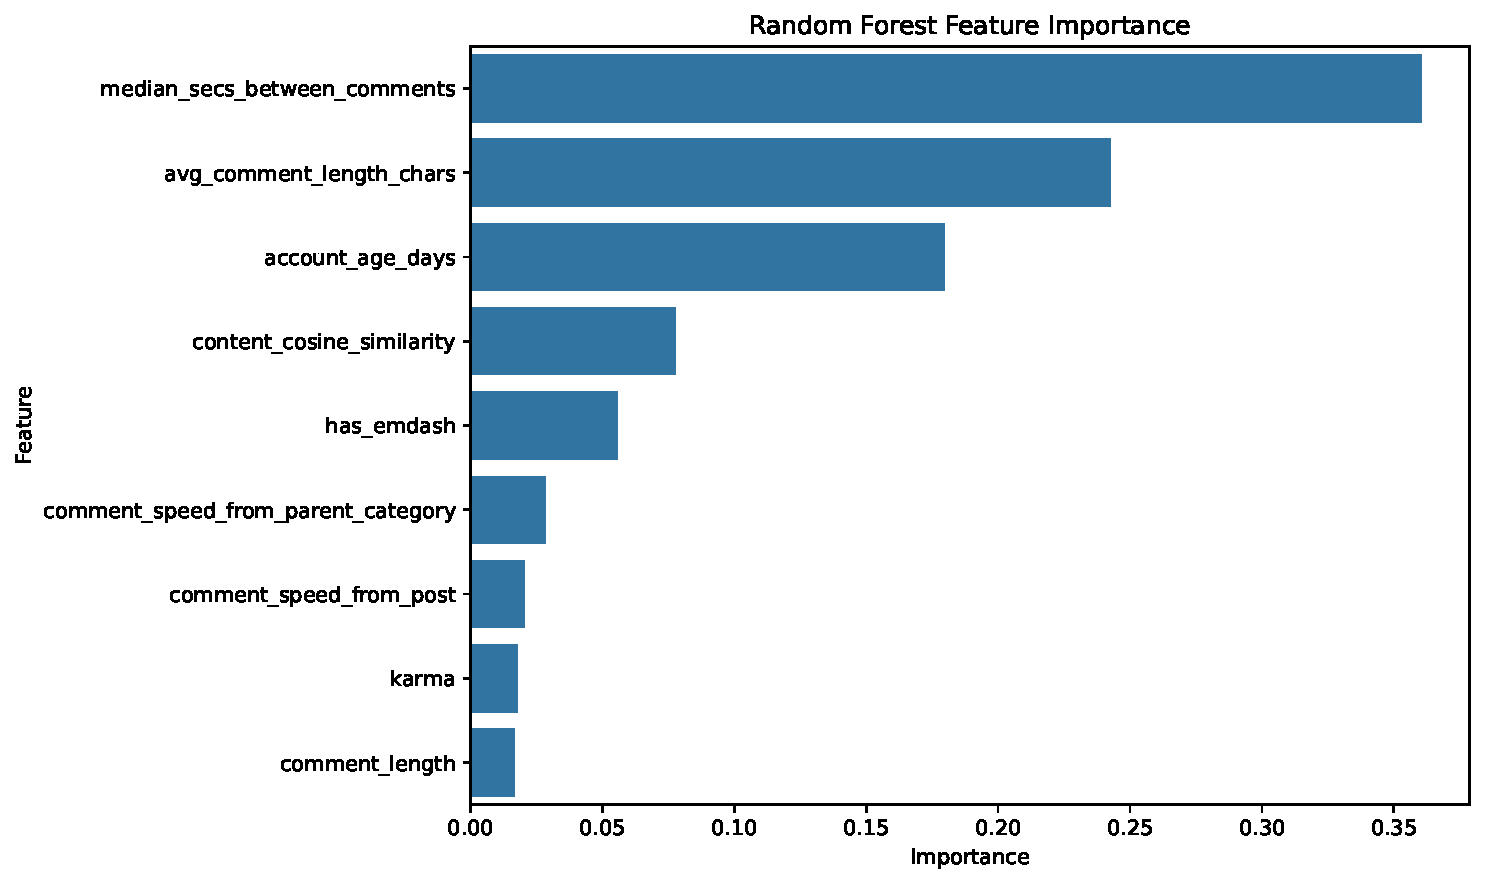
\includegraphics[width=0.85\linewidth,height=\textheight,keepaspectratio]{detecting_bots_on_reddit_code_files/figure-pdf/cell-22-output-6.pdf}

}

\caption{\label{fig-importance}Feature Importance bar chart depicting
the features that most helped the model classify each user into
categories.}

\end{figure}%

\begin{itemize}
\tightlist
\item
  \textbf{Confusion Matrices:} Figure~\ref{fig-confmat} shows the
  confusion matrix for the Random Forest classifier, which achieved the
  best performance among the tested models, as well as the other 2
  classifiers. The model exhibited a tendency to misclassify some
  non-bot accounts as bots (false positives), while achieving relatively
  better performance in correctly identifying flagged accounts (true
  positives). This suggests that the heuristic-based approach, while
  effective in identifying some bot-like accounts based on meta-metrics,
  may also inadvertently flag some legitimate, highly active users.
\end{itemize}

These quantitative results are preliminary and should be interpreted
cautiously due to the lack of a true ground truth dataset and the
limitations of relying solely on meta-metrics and basic content
features. However, they provide initial evidence supporting the
heuristic-based approach's potential for bot detection on Reddit and
highlight areas for future refinement, particularly in reducing false
positives and incorporating more sophisticated content-based features
derived from labeled data, as well as building more balanced datasets
with higher representations for what a bot may look like.

\begin{figure}

\centering{

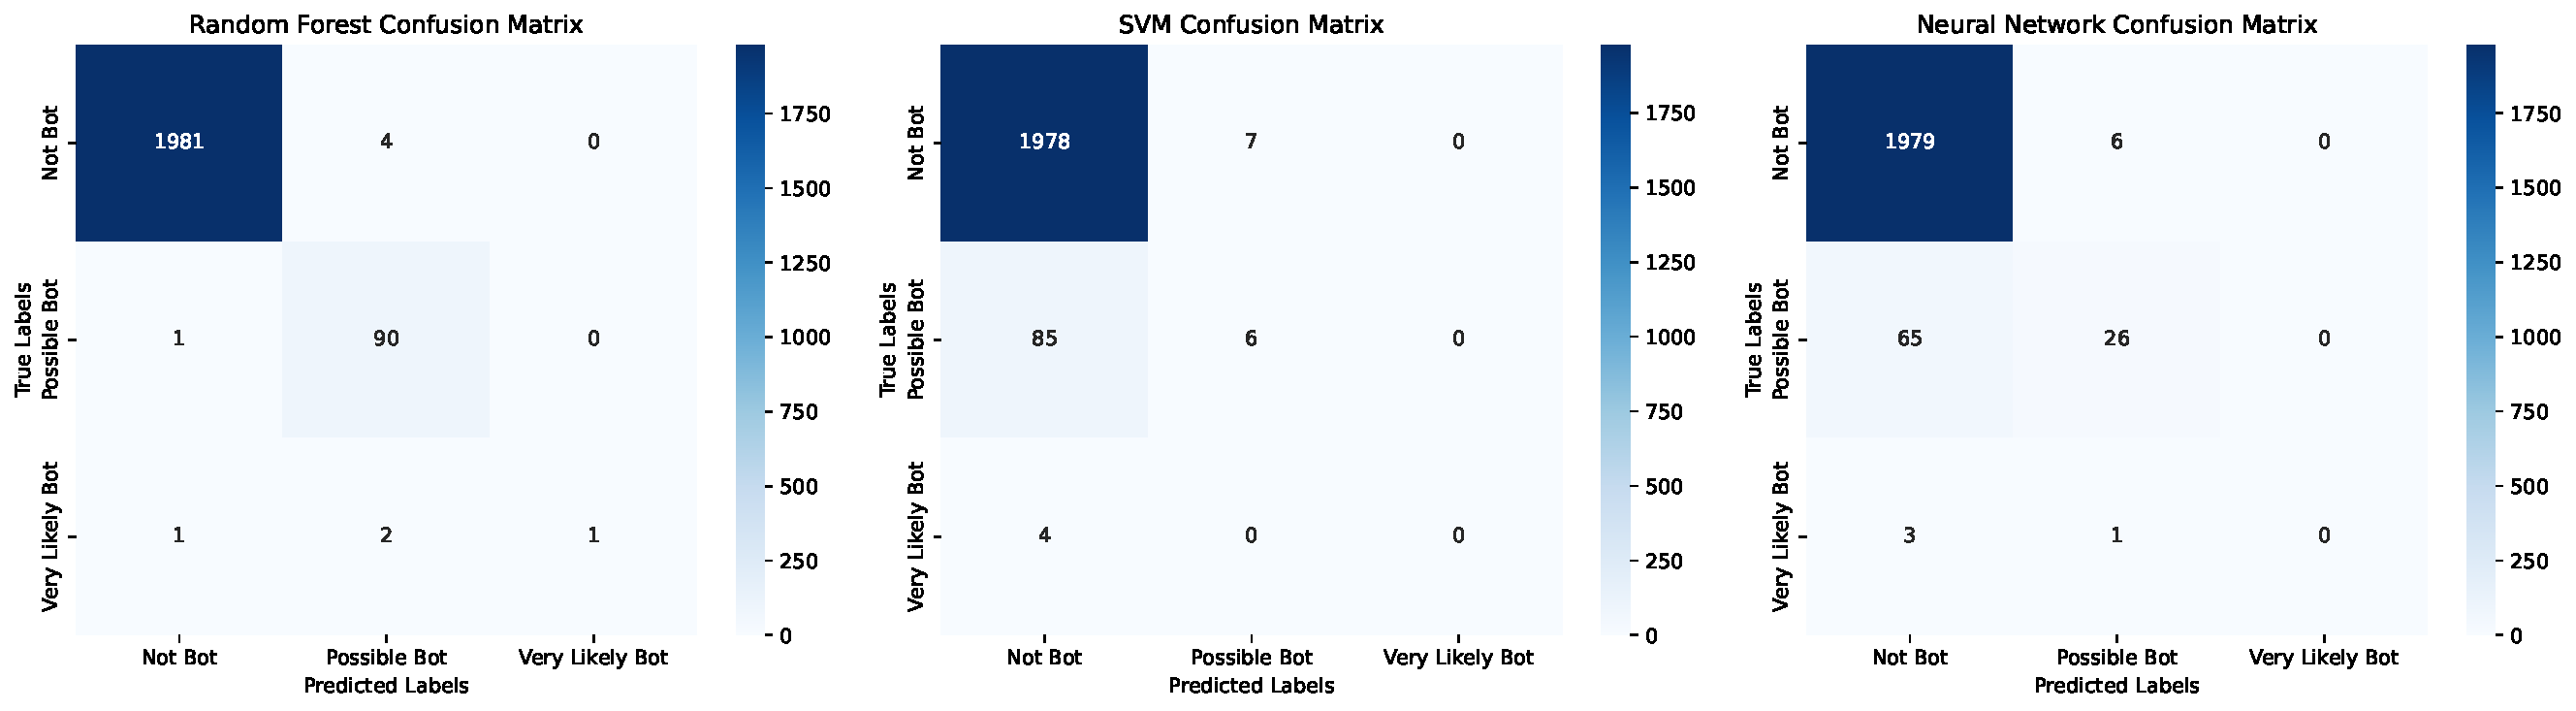
\includegraphics[width=1\linewidth,height=\textheight,keepaspectratio]{detecting_bots_on_reddit_code_files/figure-pdf/cell-22-output-5.pdf}

}

\caption{\label{fig-confmat}Confusion Matrix for each of the 3
classifiers employed in the exploratory supervised learning analysis: a
random forest left untuned is better at identifying the structures
implied by the heuristic labeling compared to the other 2 techniques we
have explored.}

\end{figure}%

\subsection{Clustering Analysis}\label{clustering-analysis}

To further explore the underlying structure of the user-level data and
visually assess potential groupings, dimensionality reduction and
clustering techniques were applied. Principal Component Analysis (PCA)
was used to reduce the dimensionality of the user-level dataset to two
principal components, allowing for visualization in a 2D space. K-Means
and DBSCAN clustering algorithms were then applied to the
PCA-transformed data to identify potential clusters of users based on
their features. The hyperparameters for each of the clustering algorithm
were selected according to the highest Average Silhouette Width.

Figure~\ref{fig-clust} displays scatter plots visualizing the results of
K-Means and DBSCAN clustering, projected onto the first two principal
components (PC1 and PC2). As shown in the figure, the visualizations
reveal some degree of clustering in the user data, although distinct,
well-separated clusters are not clearly evident.

\begin{itemize}
\item
  \textbf{K-Means Clustering:} The K-Means plot (top) shows a
  partitioning of the data into distinct clusters, but the clusters
  exhibit considerable overlap. PC1, representing a combination of
  features like average comment length, content cosine similarity, and
  comment length, is plotted on the x-axis. PC2, representing features
  like em-dash presence, karma, and median seconds between comments, is
  plotted on the y-axis. While K-Means forces data points into clusters,
  the visual overlap suggests that these clusters may not represent
  inherently distinct groups in terms of bot-like characteristics, and
  the algorithm may be imposing structure where clear separations do not
  naturally exist in the data based on these features alone.
\item
  \textbf{DBSCAN Clustering:} The DBSCAN plot (bottom) identifies a
  central dense cluster (Cluster 0, shown in yellow) and designates a
  significant portion of data points as noise (Cluster -1, shown in
  purple), indicating that these points do not belong to any
  well-defined cluster based on DBSCAN's density-based criteria. Similar
  to K-Means, the axes represent PC1 and PC2 with the same feature
  loadings. The presence of a large noise cluster further supports the
  idea that clear, distinct groupings based on bot vs.~human
  characteristics, as captured by these features and visualized in
  reduced dimensions, are not strongly present in the data. The limited
  cluster structure suggests that bot and human accounts, as identified
  by heuristics and visualized through PCA, may exist on a spectrum of
  behavioral characteristics rather than in clearly separated
  categories, at least based on the features used for clustering and
  visualization.
\end{itemize}

\begin{figure}

\centering{

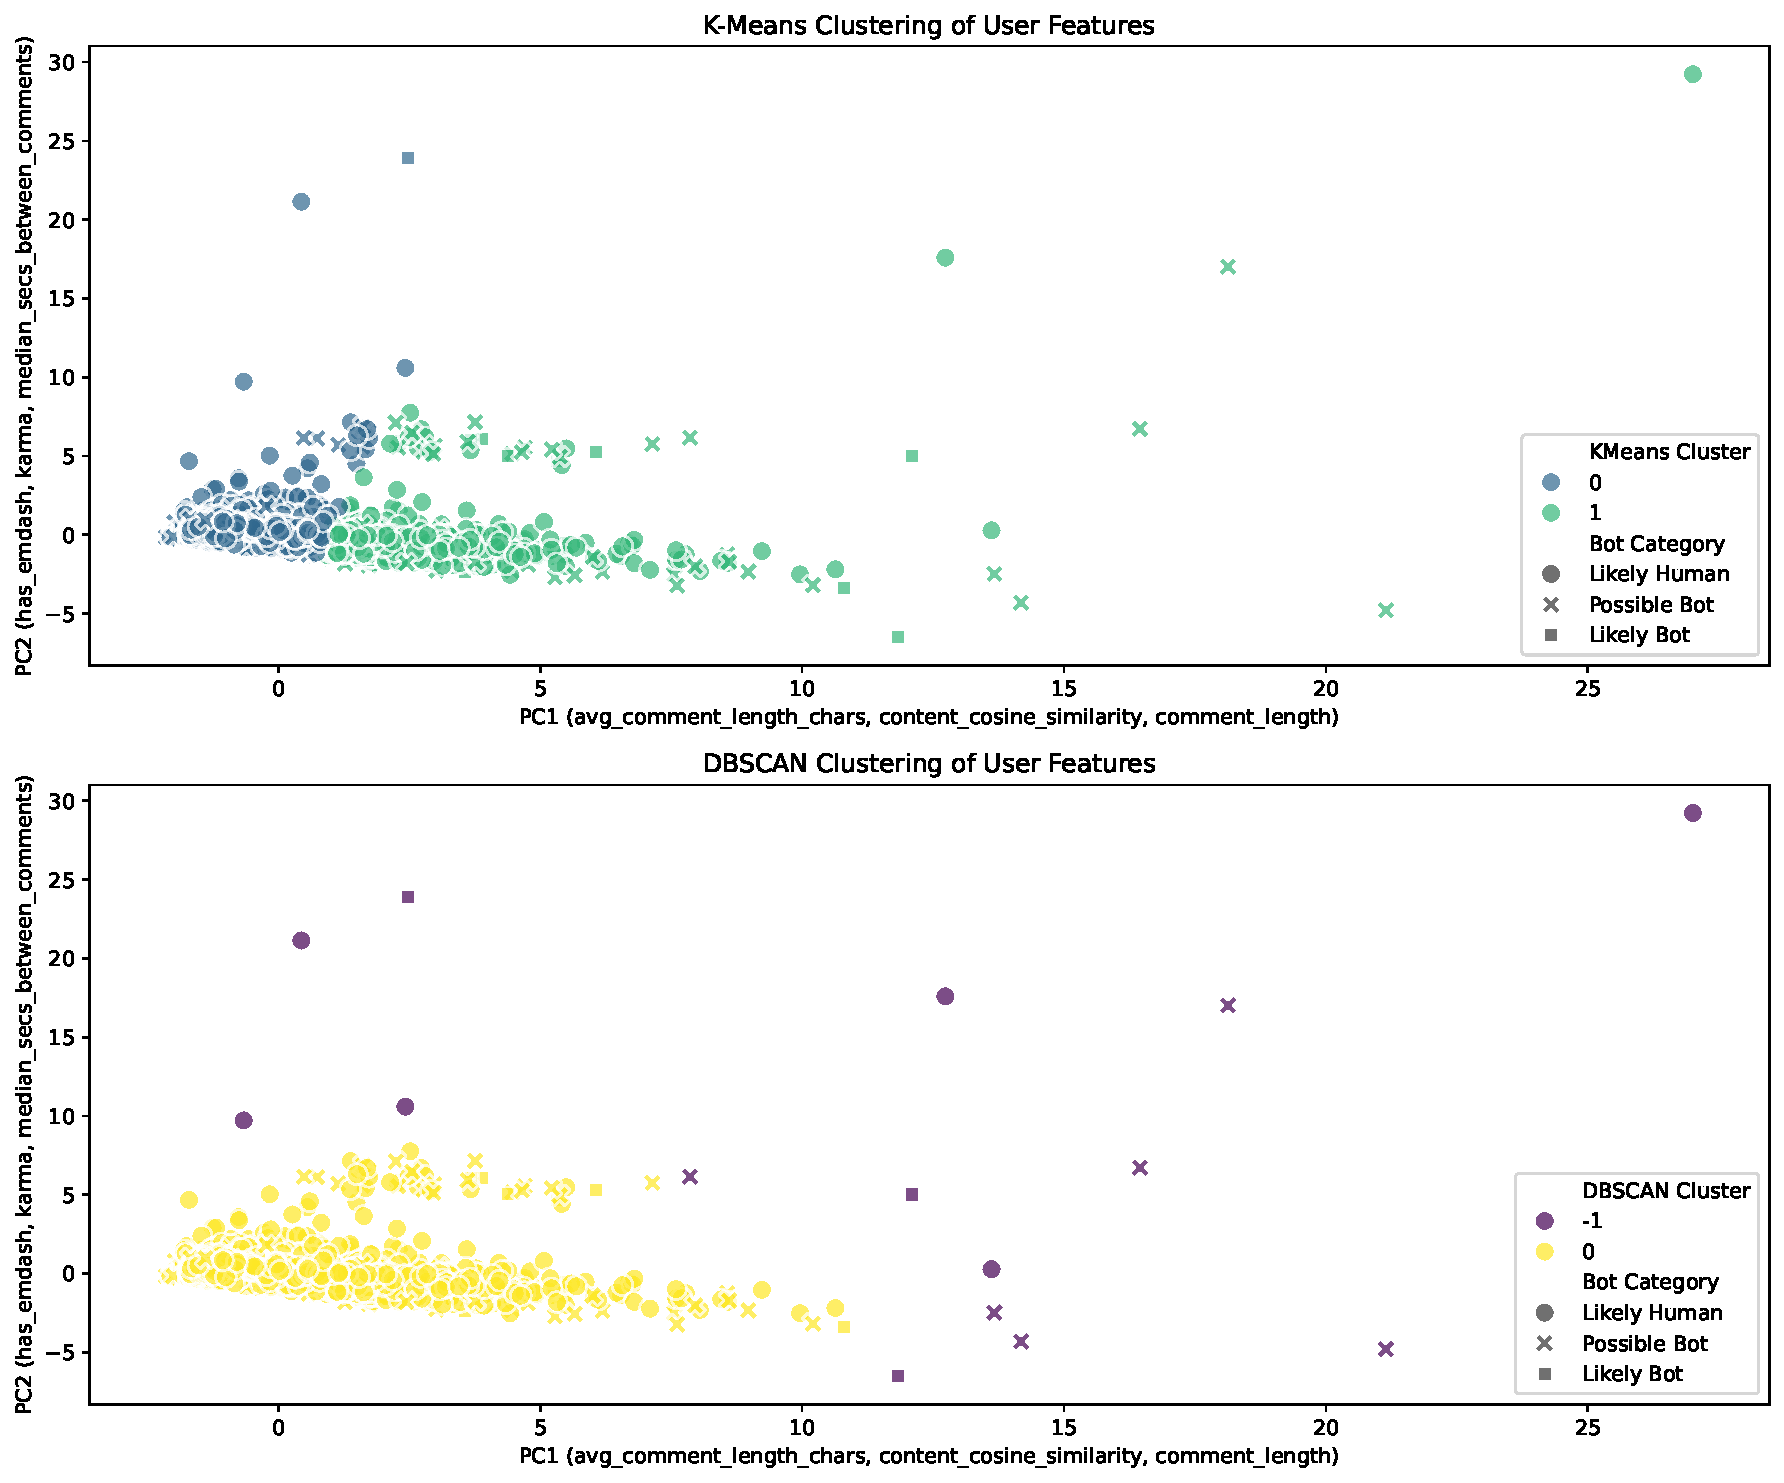
\includegraphics[width=0.85\linewidth,height=\textheight,keepaspectratio]{detecting_bots_on_reddit_code_files/figure-pdf/cell-24-output-1.pdf}

}

\caption{\label{fig-clust}K-Means and DBSCAN Clustering Visualizations:
the scatter plots visualize K-Means (top) and DBSCAN (bottom) clustering
results after PCA dimensionality reduction. Points are colored by
cluster assignment, and marker style indicates the `Bot Category'
assigned by heuristics. Axis labels indicate the top loading features
for each Principal Component.}

\end{figure}%

These clustering visualizations, while not revealing definitive bot
clusters, visually reinforce the idea that distinguishing between bots
and humans based solely on the meta-metrics and basic content features
used in this study is a complex task. The lack of clear cluster
separation suggests that more nuanced, potentially content-aware,
features and more sophisticated analytical techniques might be necessary
to effectively identify and categorize bot activity on Reddit beyond the
initial heuristic flagging.

\section{Discussion and Conclusion}\label{discussion-and-conclusion}

This study explored the feasibility of using basic heuristic methods for
detecting bot influence on Reddit discussions. The findings suggest that
simple heuristics, based on readily observable account characteristics
such as username patterns, account age, karma, posting frequency,
content repetitiveness, and em-dash presence, can effectively identify a
subset of accounts exhibiting bot-like behavior based on meta-metrics.
Descriptive analysis of flagged accounts revealed patterns consistent
with known bot characteristics, and exploratory quantitative evaluation
using machine learning classifiers provided preliminary support for the
predictive capability of the heuristic-based approach when relying on
these meta-metrics and basic content features.

\begin{figure}

\centering{

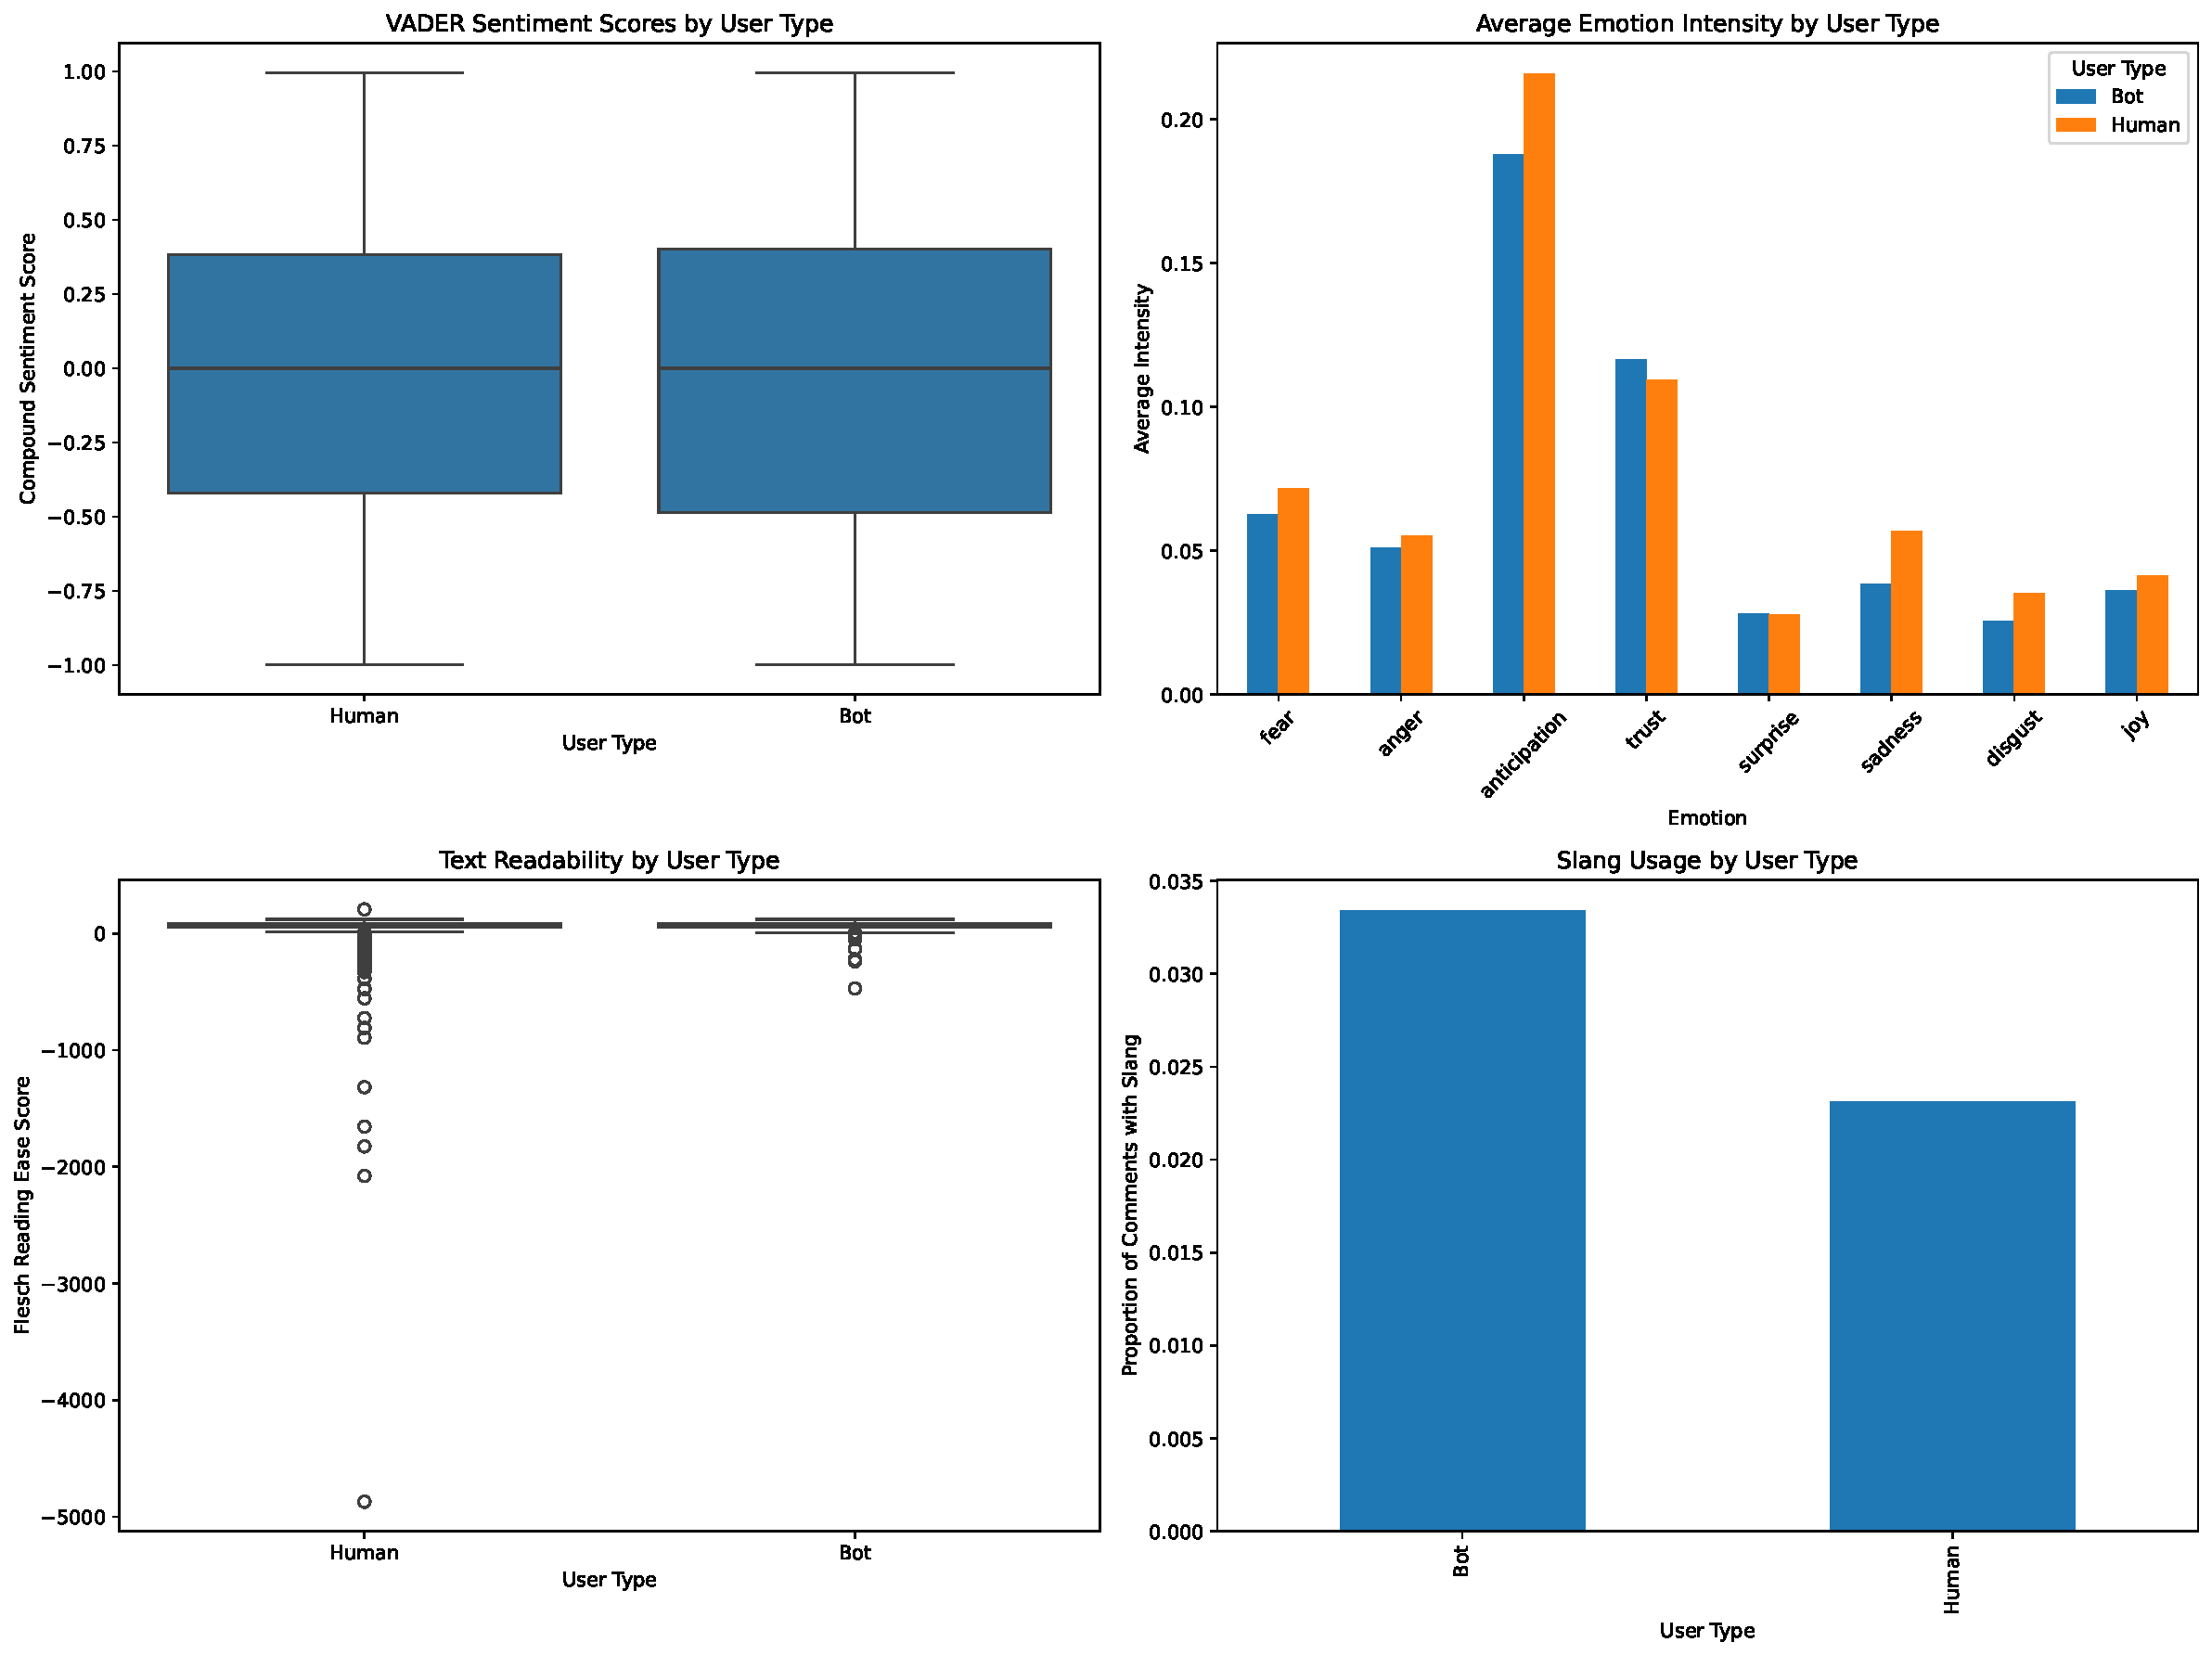
\includegraphics[width=0.85\linewidth,height=\textheight,keepaspectratio]{detecting_bots_on_reddit_code_files/figure-pdf/cell-25-output-1.pdf}

}

\caption{\label{fig-comparison}Simple metrics indicating lack of
significant differences between users labeled as likely humans
vs.~possible or likely bots. The text readability measure can be further
explored in the code file or in its original source
paper\textsuperscript{{[}\citeproc{ref-kincaid1975flesch}{30}{]}}.}

\end{figure}%

However, and importantly, the analysis of keyword frequencies and
sentiment scores did \emph{not} reveal statistically significant
differences between flagged and non-flagged accounts (see
Figure~\ref{fig-comparison}). This key finding suggests that, while
heuristic methods based on meta-metrics can identify certain bot-like
accounts, these bots may be increasingly sophisticated in mimicking
human language in terms of topical focus and sentiment expression, at
least when analyzed using simple keyword frequency and sentiment
analysis tools. This highlights a crucial limitation of relying solely
on meta-metrics and basic content analysis for bot detection in the face
of increasingly advanced automated accounts. It also suggests that
simply analyzing keyword frequencies or overall sentiment polarity may
not be sufficient to distinguish bots from humans in terms of content,
and more nuanced, context-aware content analysis methods are needed.

The study also investigated potential narrative amplification and
polarization associated with flagged accounts. While suggestive evidence
of narrative amplification was observed through keyword analysis, and
subtle differences in sentiment polarity were detected, the lack of
statistical significance in these content-based analyses underscores the
challenges in definitively attributing these phenomena to bot activity
based on the methods employed here. LLM-generated word clouds, while
thematically informative in visualizing subreddit topics, similarly did
not provide clear differentiation between bot and human language use in
terms of content.

In essence, the study demonstrates that while basic heuristics can flag
accounts exhibiting bot-like behavior, these heuristics alone are
insufficient to definitively identify bots or understand their influence
on content without more advanced content-based analysis methods and
labeled data.

\subsection{Limitations}\label{limitations}

This study has several limitations that should be considered when
interpreting the findings:

\begin{itemize}
\item
  \textbf{Heuristic Accuracy and Reliance on Meta-metrics:} The
  heuristic-based bot detection method, while interpretable and readily
  implementable, is inherently limited in its accuracy, particularly
  when relying solely on meta-metrics. It relies on predefined rules
  that may not capture the full spectrum of bot behaviors, especially
  increasingly sophisticated bots that closely mimic human users and
  whose content may be indistinguishable from human content when
  analyzed with basic
  methods\textsuperscript{{[}\citeproc{ref-botdetectionreddit}{1}{]}}.
  The exploratory quantitative evaluation revealed a tendency for false
  positives, indicating that the heuristics may inadvertently flag some
  legitimate users as bots. Crucially, the lack of significant
  differences in keyword frequencies and sentiment scores suggests that
  meta-metrics alone are insufficient for a comprehensive and nuanced
  understanding of bot activity, and that content-based analysis is
  essential for future progress.
\item
  \textbf{Lack of Ground Truth and Content Labeling:} The absence of a
  true ``ground truth'' dataset for bot identification on Reddit poses a
  significant challenge for rigorous quantitative evaluation. In none of
  the previous studies, a reasonably accurate bot detection method based
  on well-labeled data was found. Moreover, the study did not
  incorporate a crucial element for content-based bot detection: labeled
  data where comment bodies are categorized as bot-generated or
  human-generated. The exploratory machine learning evaluation provides
  only a preliminary indication of the heuristic approach's predictive
  capability based on meta-metrics but cannot definitively assess its
  accuracy against a verified bot/human classification that incorporates
  content analysis. Future research must prioritize the creation of such
  labeled datasets, potentially through human annotation or LLM-assisted
  labeling, to enable the development of more robust content-aware bot
  detection models.
\item
  \textbf{Data Sampling:} The data collection was limited to the top 50
  hottest posts per subreddit and a maximum of 2000 comments per post.
  This sampling approach may not capture the full diversity of
  discussions and bot activity across Reddit. Furthermore, the analysis
  focused on only the top 5 subreddits, limiting the generalizability of
  the findings to the entire Reddit platform.
\item
  \textbf{LLM Dependency for Exploratory Analysis:} The study's reliance
  on Google Gemini for keyword extraction and sentiment summarization,
  while providing exploratory insights, introduces a dependency on a
  specific LLM API and is not a substitute for direct content-based bot
  detection. While efforts were made to ensure reproducibility by tuning
  LLM parameters, the results should be seen as qualitative explorations
  rather than definitive quantitative measures of bot influence on
  content.
\end{itemize}

\subsection{Future Research
Directions}\label{future-research-directions}

Future research should address these limitations and further explore the
detection of bots on Reddit, with a particular emphasis on moving beyond
meta-metrics and incorporating content-based analysis:

\begin{itemize}
\item
  \textbf{Refinement of Heuristics and Integration of Content Features:}
  Further research is needed to refine and expand the heuristic-based
  bot detection method, integrating content-based features derived from
  labeled data. This could involve incorporating more sophisticated
  meta-metrics, such as network-based metrics derived from user
  interaction patterns within subreddits, but crucially, it should also
  prioritize features extracted directly from the comment text itself,
  leveraging human-validated labeled data to identify nuanced linguistic
  patterns indicative of bot-generated content, going beyond simple
  metrics like em-dash presence to encompass stylistic features,
  semantic coherence, contextual relevance, and even subtle cues in
  argumentation and conversational style. Adaptive heuristics that
  dynamically adjust to evolving bot behaviors, including content
  generation strategies, could also be explored.
\item
  \textbf{Development of Ground Truth Datasets with Human-Validated
  Content Labels:} A critical step for future research is the
  development of high-quality, labeled datasets for Reddit bot detection
  that include human-validated labels for comment content. This could
  involve combining manual labeling by expert Reddit moderators with
  LLM-assisted labeling techniques to categorize comment bodies as bot
  or human-generated, with a rigorous human review and validation
  process to ensure label accuracy and minimize biases. This labeled
  data is essential to train and evaluate models that can effectively
  leverage content-based features for bot detection, moving beyond the
  limitations of meta-metrics and basic content features.
\item
  \textbf{Advanced Machine Learning Models for Content-Aware Bot
  Detection:} Future studies should investigate the application of more
  advanced machine learning models, trained on datasets with
  human-validated content labels, for Reddit bot detection. These
  models, capable of processing and understanding natural language, may
  be better suited to capture the complex behavioral and linguistic
  patterns of sophisticated bots and potentially improve detection
  accuracy by learning directly from the content of bot and human
  comments, going beyond simple keyword or sentiment analysis to
  understand deeper semantic, stylistic, and contextual cues that
  differentiate human and bot-generated text.
\item
  \textbf{Hybrid Approaches Combining Meta-metrics and Content
  Analysis:} Combining heuristic-based methods, focused on meta-metrics,
  with machine learning models trained on content-labeled data could
  offer a promising avenue for future research. Heuristics could be used
  for initial feature engineering and data pre-processing of meta-data,
  while machine learning models could be trained to learn more complex
  patterns and improve detection accuracy by incorporating both
  meta-metric and content-based features derived from human-validated
  labeled data, creating a more robust and nuanced bot detection system
  that leverages the strengths of both rule-based and data-driven
  approaches.
\end{itemize}

\subsection{Conclusion}\label{conclusion}

This study provides a preliminary exploration into the detection of bots
on Reddit using basic heuristic methods and LLMs for exploratory
analysis. While heuristic-based approaches offer a readily implementable
and interpretable starting point for identifying some bot-like accounts
based on meta-metrics, the study highlights the crucial limitation of
relying solely on meta-metrics and basic content analysis in the face of
increasingly sophisticated bots. The key takeaway is the necessity of
moving beyond meta-metrics and incorporating human-validated
content-based analysis, which requires the development of labeled
datasets and the application of advanced machine learning models capable
of understanding and learning from the textual content of Reddit
comments, while carefully considering ethical implications and ensuring
fairness and transparency. Future research must prioritize these
directions to develop more robust, accurate, ethically sound, and
content-aware bot detection systems for this complex and evolving online
environment. The ongoing effort to detect and mitigate bot influence,
particularly through advanced content-aware methods, is crucial for
maintaining the integrity and trustworthiness of online social platforms
and ensuring a healthy digital public sphere.

\newpage

\section*{References}\label{references}
\addcontentsline{toc}{section}{References}

\phantomsection\label{refs}
\begin{CSLReferences}{1}{0}
\bibitem[\citeproctext]{ref-botdetectionreddit}
1. Hurtado S., Ray P., \& Marculescu R. (2019). Bot detection in reddit
political discussion. \emph{ResearchGate}.
\url{https://www.researchgate.net/publication/332340547_Bot_Detection_in_Reddit_Political_Discussion}

\bibitem[\citeproctext]{ref-redditbotproblem}
2. Dawson A. (2024). Does reddit have a bot problem? absolutely. In
\emph{Lunio}. \url{https://www.lunio.ai/blog/reddit-bots}

\bibitem[\citeproctext]{ref-redditbotwatch}
3. R/botwatch. (2022). In \emph{Reddit}.
\url{https://www.reddit.com/r/botwatch/}

\bibitem[\citeproctext]{ref-multibotdetector}
4. Ng L. H. X., \& Carley K. M. (2022). Assembling a multi-platform
ensemble social bot detector with applications to US 2020 elections.
\emph{arXiv}. \url{https://arxiv.org/html/2401.14607v1}

\bibitem[\citeproctext]{ref-breiman2001random}
5. Breiman L. (2001). Random forests. \emph{Machine Learning},
\emph{45}(1), 5--32. \url{https://doi.org/10.1023/A:1010933404324}

\bibitem[\citeproctext]{ref-breiman1984classification}
6. Breiman L., Friedman J. H., Olshen R. A., \& Stone C. J. (1984).
\emph{Classification and regression trees}. Wadsworth International
Group.

\bibitem[\citeproctext]{ref-evalsocialbotmodels}
7. Kutlu M., \& Selçuk A. A. (2025). Evaluation of social bot detection
models. \emph{ResearchGate}.
\url{https://www.researchgate.net/publication/361038547_Evaluation_of_social_bot_detection_models}

\bibitem[\citeproctext]{ref-hochreiter1997long}
8. Hochreiter S., \& Schmidhuber J. (1997). Long short-term memory.
\emph{Neural Computation}, \emph{9}(8), 1735--1780.
\url{https://doi.org/10.1162/neco.1997.9.8.1735}

\bibitem[\citeproctext]{ref-dietterich2000ensemble}
9. Dietterich T. G. (2000). \emph{Ensemble methods in machine learning}.
1--15.

\bibitem[\citeproctext]{ref-anomalycloudflare}
10. Tang J. (2024). \emph{Lessons learned from scaling up cloudflare's
anomaly detection platform}.
\url{https://blog.cloudflare.com/lessons-learned-from-scaling-up-cloudflare-anomaly-detection-platform/}

\bibitem[\citeproctext]{ref-anomalyf5networks}
11. Tang J. (2024). How does anomaly detection work? : R/f5networks. In
\emph{Reddit}.
\url{https://www.reddit.com/r/f5networks/comments/13jw4qg/how_does_anomaly_detection_work/}

\bibitem[\citeproctext]{ref-chandola2009anomaly}
12. Chandola V., Banerjee A., \& Kumar V. (2009). Anomaly detection: A
survey. \emph{ACM Computing Surveys (CSUR)}, \emph{41}(3), 1--58.
\url{https://doi.org/10.1145/1541880.1541882}

\bibitem[\citeproctext]{ref-goldstein2012histogram}
13. Goldstein M., \& Dengel A. (2012). Histogram-based outlier score
(HBOS): A fast unsupervised anomaly detection algorithm. \emph{KI-2012:
Poster and Demo Track}, 59--63.

\bibitem[\citeproctext]{ref-redditbotnetwork}
14. Damasceno R. (2019). Identify-bots-reddit-comment-network:
Characterization and classification of bots using only structural
characteristics of the network. In \emph{GitHub}.
\url{https://github.com/DamascenoRafael/identify-bots-reddit-comment-network}

\bibitem[\citeproctext]{ref-mlredditbots}
15. Skowronski J. (2019). Identifying trolls and bots on reddit with
machine learning. In \emph{Medium}.
\url{https://medium.com/towards-data-science/identifying-trolls-and-bots-on-reddit-with-machine-learning-709da5970af1}

\bibitem[\citeproctext]{ref-pushshiftredditdataset}
16. Baumgartner J., Zannettou S., Keegan B., Squire M., \& Blackburn J.
(2020). The pushshift reddit dataset. \emph{AAAI Publications}.
\url{https://ojs.aaai.org/index.php/ICWSM/article/view/7347/7201}

\bibitem[\citeproctext]{ref-redditcommentsdataset}
17. Tkachenko V. (2021). Reddit comments dataset. In \emph{ClickHouse
Docs}.
\url{https://clickhouse.com/docs/getting-started/example-datasets/reddit-comments}

\bibitem[\citeproctext]{ref-praw2024}
18. Reddit. (2024). \emph{{PRAW}: Python reddit API wrapper}.
\url{https://praw.readthedocs.io/en/stable/}

\bibitem[\citeproctext]{ref-googleai2023gemini}
19. Google. (2023). \emph{Gemini API}.
\url{https://ai.google.dev/products/gemini}

\bibitem[\citeproctext]{ref-redditbotdetector}
20. Tourond M. (2019). Reddit-bot-detector: A python bot that detects
reddit bots. In \emph{GitHub}.
\url{https://github.com/MatthewTourond/Reddit-Bot-Detector}

\bibitem[\citeproctext]{ref-originalityaiblog}
21. Gillham J., \& Lambert M. (2023). \emph{Are you getting advice from
a human or bot? Reddit shows spikes in AI content}.
\url{https://originality.ai/blog/reddit-shows-spikes-in-ai-content}

\bibitem[\citeproctext]{ref-nightwateremdash}
22. Bush C. (2023). \emph{The em dash and AI: A conjunction - night
water}. \url{https://www.nightwater.email/em-dash-ai/}

\bibitem[\citeproctext]{ref-redditbotslearnusetalents}
23. How to identify bots on reddit : R/LearnUselessTalents. (2023). In
\emph{Reddit}.
\url{https://www.reddit.com/r/LearnUselessTalents/comments/15tzjkb/how_to_identify_bots_on_reddit/}

\bibitem[\citeproctext]{ref-botsidentifytyrannosnorlax}
24. u/tyrannosnorlax. (2022). Bots. How to identify them, and why do
they exist on reddit? In \emph{Reddit}.
\url{https://www.reddit.com/user/tyrannosnorlax/comments/t0h466/bots_how_to_identify_them_and_why_do_they_exist/}

\bibitem[\citeproctext]{ref-botproblem7daystodie}
25. Bot problem - how to identify bot accounts (99\% accuracy) :
R/7daystodie. (2025). In \emph{Reddit}.
\url{https://www.reddit.com/r/7daystodie/comments/1au1g1s/bot_problem_how_to_identify_bot_accounts_99/}

\bibitem[\citeproctext]{ref-hutto2014vader}
26. Hutto C. J., \& Gilbert E. (2014). \emph{VADER: A parsimonious
rule-based model for sentiment analysis of social media text}.
\url{http://comp.social.gatech.edu/papers/icwsm14.vader.hutto.pdf}

\bibitem[\citeproctext]{ref-cortes1995support}
27. Cortes C., \& Vapnik V. (1995). Support-vector networks.
\emph{Machine Learning}, \emph{20}(3), 273--297.
\url{https://doi.org/10.1007/BF00994018}

\bibitem[\citeproctext]{ref-lecun2015deep}
28. LeCun Y., Bengio Y., \& Hinton G. (2015). Deep learning.
\emph{Nature}, \emph{521}(7553), 436--444.
\url{https://doi.org/10.1038/nature14539}

\bibitem[\citeproctext]{ref-salton1988term}
29. Salton G., \& Buckley C. (1988). Term-weighting approaches in
automatic text retrieval. \emph{Information Processing \& Management},
\emph{24}(5), 513--523.
\url{https://doi.org/10.1016/0306-4573(88)90021-0}

\bibitem[\citeproctext]{ref-kincaid1975flesch}
30. Kincaid J. P., Fishburne Jr R. P., Rogers R. L., \& Chissom B. S.
(1975). \emph{Derivation of new readability formulas (automated
readability index, fog count and flesch reading ease formula) for navy
enlisted personnel}.

\end{CSLReferences}

\newpage

\section*{Appendix}\label{appendix}
\addcontentsline{toc}{section}{Appendix}

\subsection*{Keyword Generation and Subreddit Selection
Details}\label{keyword-generation-and-subreddit-selection-details}
\addcontentsline{toc}{subsection}{Keyword Generation and Subreddit
Selection Details}

\begin{Shaded}
\begin{Highlighting}[]
\CommentTok{\# Fetch a large subset of popular subreddits (large limit makes this representative of the largest overall subreddits by subscribers, check: https://gummysearch.com/tools/top{-}subreddits/)}
\NormalTok{subreddits }\OperatorTok{=} \BuiltInTok{list}\NormalTok{(reddit.subreddits.popular(limit}\OperatorTok{=}\DecValTok{1000}\NormalTok{))}

\CommentTok{\# Create a DataFrame using list comprehension for better performance}
\NormalTok{subs\_df }\OperatorTok{=}\NormalTok{ pd.DataFrame([\{}
    \StringTok{"Name"}\NormalTok{: subreddit.display\_name,}
    \StringTok{"Subscribers"}\NormalTok{: subreddit.subscribers,}
    \StringTok{"Description"}\NormalTok{: subreddit.public\_description,}
    \StringTok{"Over 18"}\NormalTok{: subreddit.over18,}
    \StringTok{"Submission Type"}\NormalTok{: subreddit.submission\_type}
\NormalTok{\} }\ControlFlowTok{for}\NormalTok{ subreddit }\KeywordTok{in}\NormalTok{ subreddits]).sort\_values(by}\OperatorTok{=}\StringTok{"Subscribers"}\NormalTok{, ascending}\OperatorTok{=}\VariableTok{False}\NormalTok{, ignore\_index}\OperatorTok{=}\VariableTok{True}\NormalTok{)}

\CommentTok{\# Print the top 10}
\NormalTok{subs\_df.head(}\DecValTok{10}\NormalTok{)}
\end{Highlighting}
\end{Shaded}

\begin{longtable}[]{@{}llllll@{}}
\toprule\noalign{}
& Name & Subscribers & ... & Over 18 & Submission Type \\
\midrule\noalign{}
\endhead
\bottomrule\noalign{}
\endlastfoot
0 & funny & 66606333 & ... & False & any \\
1 & AskReddit & 53187135 & ... & False & self \\
2 & gaming & 46011600 & ... & False & any \\
3 & worldnews & 44854924 & ... & False & link \\
4 & todayilearned & 40129819 & ... & False & link \\
5 & aww & 37646001 & ... & False & link \\
6 & Music & 36997898 & ... & False & any \\
7 & memes & 35398685 & ... & False & link \\
8 & movies & 34857549 & ... & False & any \\
9 & Showerthoughts & 34153828 & ... & False & self \\
\end{longtable}

\begin{Shaded}
\begin{Highlighting}[]
\ImportTok{import}\NormalTok{ ast}

\NormalTok{response }\OperatorTok{=}\NormalTok{ generate(}\StringTok{"What are some keywords I can use to create a list of subreddits which are likely to be influenced by bots because of their controversial nature? These are keywords that I would look for within a subreddit\textquotesingle{}s name or description. For example: }\CharTok{\textbackslash{}"}\StringTok{news}\CharTok{\textbackslash{}"}\StringTok{, }\CharTok{\textbackslash{}"}\StringTok{politics}\CharTok{\textbackslash{}"}\StringTok{, }\CharTok{\textbackslash{}"}\StringTok{discussion}\CharTok{\textbackslash{}"}\StringTok{, }\CharTok{\textbackslash{}"}\StringTok{war}\CharTok{\textbackslash{}"}\StringTok{, }\CharTok{\textbackslash{}"}\StringTok{vaccines}\CharTok{\textbackslash{}"}\StringTok{, }\CharTok{\textbackslash{}"}\StringTok{controversial}\CharTok{\textbackslash{}"}\StringTok{, }\CharTok{\textbackslash{}"}\StringTok{conflict}\CharTok{\textbackslash{}"}\StringTok{, etc.}\CharTok{\textbackslash{}n\textbackslash{}n}\StringTok{Keep the answer short, only including 50 keywords and saving them in a python list as follows [}\CharTok{\textbackslash{}"}\StringTok{key1}\CharTok{\textbackslash{}"}\StringTok{,}\CharTok{\textbackslash{}"}\StringTok{key2}\CharTok{\textbackslash{}"}\StringTok{,...]. Send the output as text not as code."}\NormalTok{)}

\NormalTok{bot\_influence\_keywords }\OperatorTok{=}\NormalTok{ ast.literal\_eval(response.replace(}\StringTok{"}\CharTok{\textbackslash{}n}\StringTok{"}\NormalTok{, }\StringTok{""}\NormalTok{))}

\ControlFlowTok{for}\NormalTok{ i }\KeywordTok{in} \BuiltInTok{range}\NormalTok{(}\DecValTok{0}\NormalTok{, }\BuiltInTok{len}\NormalTok{(bot\_influence\_keywords), }\DecValTok{5}\NormalTok{):}
    \BuiltInTok{print}\NormalTok{(}\OperatorTok{*}\NormalTok{bot\_influence\_keywords[i:i}\OperatorTok{+}\DecValTok{5}\NormalTok{])}
\end{Highlighting}
\end{Shaded}

\begin{verbatim}
news politics discussion war vaccines
controversial conflict debate election government
russia china ukraine israel palestine
climate immigration guns religion socialism
capitalism feminism lgbt transgender race
identity activism protest censorship freedom
rights justice police crime law
economy finance markets technology science
health global world opinion truth
facts bias propaganda conspiracy agenda
\end{verbatim}

\begin{Shaded}
\begin{Highlighting}[]
\CommentTok{\# Score subreddits based on subscribers and keywords in description}
\KeywordTok{def}\NormalTok{ calculate\_bot\_influence\_score(row):}
\NormalTok{    score }\OperatorTok{=} \DecValTok{0}
    
    \CommentTok{\# Large subscriber base increases potential for bot activity}
    \ControlFlowTok{if}\NormalTok{ row[}\StringTok{\textquotesingle{}Subscribers\textquotesingle{}}\NormalTok{] }\OperatorTok{\textgreater{}} \DecValTok{10000000}\NormalTok{:}
\NormalTok{        score }\OperatorTok{+=} \DecValTok{5}
    \ControlFlowTok{elif}\NormalTok{ row[}\StringTok{\textquotesingle{}Subscribers\textquotesingle{}}\NormalTok{] }\OperatorTok{\textgreater{}} \DecValTok{5000000}\NormalTok{:}
\NormalTok{        score }\OperatorTok{+=} \DecValTok{4}
    \ControlFlowTok{elif}\NormalTok{ row[}\StringTok{\textquotesingle{}Subscribers\textquotesingle{}}\NormalTok{] }\OperatorTok{\textgreater{}} \DecValTok{1000000}\NormalTok{:}
\NormalTok{        score }\OperatorTok{+=} \DecValTok{3}
        
    \CommentTok{\# Check for keywords in description and subreddit name}
\NormalTok{    description }\OperatorTok{=}\NormalTok{ row[}\StringTok{\textquotesingle{}Description\textquotesingle{}}\NormalTok{].lower()}
\NormalTok{    sub\_name }\OperatorTok{=}\NormalTok{ row[}\StringTok{\textquotesingle{}Name\textquotesingle{}}\NormalTok{].lower()}
    \ControlFlowTok{for}\NormalTok{ keyword }\KeywordTok{in}\NormalTok{ bot\_influence\_keywords:}
        \ControlFlowTok{if}\NormalTok{ keyword }\KeywordTok{in}\NormalTok{ description:}
\NormalTok{            score }\OperatorTok{+=} \DecValTok{1}
        \ControlFlowTok{if}\NormalTok{ keyword }\KeywordTok{in}\NormalTok{ sub\_name:}
\NormalTok{            score }\OperatorTok{+=} \DecValTok{1}
            
    \ControlFlowTok{return}\NormalTok{ score}

\NormalTok{subs\_df[}\StringTok{\textquotesingle{}Bot Score\textquotesingle{}}\NormalTok{] }\OperatorTok{=}\NormalTok{ subs\_df.}\BuiltInTok{apply}\NormalTok{(calculate\_bot\_influence\_score, axis}\OperatorTok{=}\DecValTok{1}\NormalTok{)}

\CommentTok{\# Get top 50 most vulnerable subreddits}
\NormalTok{top\_vulnerable }\OperatorTok{=}\NormalTok{ subs\_df.nlargest(}\DecValTok{50}\NormalTok{, }\StringTok{\textquotesingle{}Bot Score\textquotesingle{}}\NormalTok{)[[}\StringTok{\textquotesingle{}Name\textquotesingle{}}\NormalTok{, }\StringTok{\textquotesingle{}Subscribers\textquotesingle{}}\NormalTok{, }\StringTok{\textquotesingle{}Submission Type\textquotesingle{}}\NormalTok{, }\StringTok{\textquotesingle{}Bot Score\textquotesingle{}}\NormalTok{]].reset\_index(drop}\OperatorTok{=}\VariableTok{True}\NormalTok{)}
\NormalTok{top\_vulnerable.head(}\DecValTok{10}\NormalTok{)}
\end{Highlighting}
\end{Shaded}

\begin{longtable}[]{@{}lllll@{}}
\toprule\noalign{}
& Name & Subscribers & Submission Type & Bot Score \\
\midrule\noalign{}
\endhead
\bottomrule\noalign{}
\endlastfoot
0 & worldnews & 44854924 & link & 9 \\
1 & technology & 18525637 & link & 9 \\
2 & IndiaSpeaks & 1049500 & any & 9 \\
3 & news & 29805254 & link & 8 \\
4 & pcmasterrace & 14768233 & any & 8 \\
5 & politics & 8785629 & link & 8 \\
6 & movies & 34857549 & any & 7 \\
7 & science & 33806399 & link & 7 \\
8 & askscience & 26054617 & self & 7 \\
9 & AmItheAsshole & 24119019 & self & 7 \\
\end{longtable}

\subsection*{Prompt for LLM-based Word Clouds and Sentiment
Analysis}\label{prompt-for-llm-based-word-clouds-and-sentiment-analysis}
\addcontentsline{toc}{subsection}{Prompt for LLM-based Word Clouds and
Sentiment Analysis}

\begin{Shaded}
\begin{Highlighting}[]
\ImportTok{import}\NormalTok{ os}
\ImportTok{import}\NormalTok{ pandas }\ImportTok{as}\NormalTok{ pd}
\ImportTok{import}\NormalTok{ matplotlib.pyplot }\ImportTok{as}\NormalTok{ plt}
\ImportTok{from}\NormalTok{ google }\ImportTok{import}\NormalTok{ genai}
\ImportTok{from}\NormalTok{ google.genai }\ImportTok{import}\NormalTok{ types}
\ImportTok{from}\NormalTok{ wordcloud }\ImportTok{import}\NormalTok{ WordCloud}
\ImportTok{import}\NormalTok{ random}

\CommentTok{\# {-}{-}{-}{-}{-} Step 1: Extract Top 5 Subreddits from ml\_features {-}{-}{-}{-}{-}}
\CommentTok{\# Assume ml\_features is already in your environment.}
\NormalTok{top\_subreddits }\OperatorTok{=}\NormalTok{ ml\_features[}\StringTok{\textquotesingle{}subreddit\textquotesingle{}}\NormalTok{].value\_counts().head(}\DecValTok{5}\NormalTok{).index.tolist()}

\CommentTok{\# {-}{-}{-}{-}{-} Step 2: Stratified Sampling {-}{-}{-}{-}{-} }
\NormalTok{sampled\_comments }\OperatorTok{=}\NormalTok{ \{\}}
\NormalTok{sample\_size }\OperatorTok{=} \DecValTok{100}
\ControlFlowTok{for}\NormalTok{ subreddit }\KeywordTok{in}\NormalTok{ top\_subreddits:}
\NormalTok{    subreddit\_comments }\OperatorTok{=}\NormalTok{ ml\_features[ml\_features[}\StringTok{\textquotesingle{}subreddit\textquotesingle{}}\NormalTok{] }\OperatorTok{==}\NormalTok{ subreddit][}\StringTok{\textquotesingle{}comment\_body\textquotesingle{}}\NormalTok{]}
    \ControlFlowTok{if} \BuiltInTok{len}\NormalTok{(subreddit\_comments) }\OperatorTok{\textgreater{}}\NormalTok{ sample\_size:}
\NormalTok{        sampled }\OperatorTok{=}\NormalTok{ subreddit\_comments.sample(n}\OperatorTok{=}\NormalTok{sample\_size, random\_state}\OperatorTok{=}\DecValTok{42}\NormalTok{)}
    \ControlFlowTok{else}\NormalTok{:}
\NormalTok{        sampled }\OperatorTok{=}\NormalTok{ subreddit\_comments}
\NormalTok{    sampled\_comments[subreddit] }\OperatorTok{=}\NormalTok{ sampled.tolist()}

\CommentTok{\# {-}{-}{-}{-}{-} Step 3: Gemini API generate() Function {-}{-}{-}{-}{-}}
\KeywordTok{def}\NormalTok{ generate(prompt):}
\NormalTok{    client }\OperatorTok{=}\NormalTok{ genai.Client(}
\NormalTok{        api\_key}\OperatorTok{=}\NormalTok{os.getenv(}\StringTok{"GEMINI\_API\_KEY"}\NormalTok{),}
\NormalTok{    )}
\NormalTok{    model }\OperatorTok{=} \StringTok{"gemini{-}2.0{-}flash"}
\NormalTok{    contents }\OperatorTok{=}\NormalTok{ [}
\NormalTok{        types.Content(}
\NormalTok{            role}\OperatorTok{=}\StringTok{"user"}\NormalTok{,}
\NormalTok{            parts}\OperatorTok{=}\NormalTok{[}
\NormalTok{                types.Part.from\_text(text}\OperatorTok{=}\NormalTok{prompt),}
\NormalTok{            ],}
\NormalTok{        ),}
\NormalTok{    ]}
\NormalTok{    generate\_content\_config }\OperatorTok{=}\NormalTok{ types.GenerateContentConfig(}
\NormalTok{        temperature}\OperatorTok{=}\DecValTok{0}\NormalTok{,}
\NormalTok{        top\_p}\OperatorTok{=}\DecValTok{0}\NormalTok{,}
\NormalTok{        top\_k}\OperatorTok{=}\DecValTok{1}\NormalTok{,}
\NormalTok{        max\_output\_tokens}\OperatorTok{=}\DecValTok{8192}\NormalTok{,}
\NormalTok{        response\_mime\_type}\OperatorTok{=}\StringTok{"text/plain"}\NormalTok{,}
\NormalTok{    )}
\NormalTok{    complete\_response }\OperatorTok{=} \StringTok{""}
    \ControlFlowTok{for}\NormalTok{ chunk }\KeywordTok{in}\NormalTok{ client.models.generate\_content\_stream(}
\NormalTok{        model}\OperatorTok{=}\NormalTok{model,}
\NormalTok{        contents}\OperatorTok{=}\NormalTok{contents,}
\NormalTok{        config}\OperatorTok{=}\NormalTok{generate\_content\_config,}
\NormalTok{    ):}
\NormalTok{        complete\_response }\OperatorTok{+=}\NormalTok{ chunk.text}
    \ControlFlowTok{return}\NormalTok{ complete\_response.strip()}

\CommentTok{\# {-}{-}{-}{-}{-} Step 4: Query the LLM for Each Subreddit {-}{-}{-}{-}{-}}
\NormalTok{subreddit\_responses }\OperatorTok{=}\NormalTok{ \{\}}
\ControlFlowTok{for}\NormalTok{ subreddit, comments }\KeywordTok{in}\NormalTok{ sampled\_comments.items():}
    \CommentTok{\# Take a random sample of comments if there are too many}
    \ControlFlowTok{if} \BuiltInTok{len}\NormalTok{(}\StringTok{" "}\NormalTok{.join(comments)) }\OperatorTok{\textgreater{}} \DecValTok{4000}\NormalTok{:}
\NormalTok{        random.seed(}\DecValTok{42}\NormalTok{)  }\CommentTok{\# For reproducibility}
\NormalTok{        sampled\_comments }\OperatorTok{=}\NormalTok{ random.sample(comments, }\BuiltInTok{min}\NormalTok{(}\BuiltInTok{len}\NormalTok{(comments), }\DecValTok{50}\NormalTok{))}
\NormalTok{        text\_blob }\OperatorTok{=} \StringTok{" "}\NormalTok{.join(sampled\_comments)[:}\DecValTok{4000}\NormalTok{]}
    \ControlFlowTok{else}\NormalTok{:}
\NormalTok{        text\_blob }\OperatorTok{=} \StringTok{" "}\NormalTok{.join(comments)[:}\DecValTok{4000}\NormalTok{]}
\NormalTok{    prompt }\OperatorTok{=}\NormalTok{ (}
        \SpecialStringTok{f"Perform sentiment analysis on the following comments from subreddit /r/}\SpecialCharTok{\{}\NormalTok{subreddit}\SpecialCharTok{\}}\SpecialStringTok{. "}
        \StringTok{"Identify 20 unique keywords (based exclusively on the text you are fed) that capture the essence of this subreddit (which can later be used for word clouds), and provide a brief sentiment summary (e.g. note if the overall tone is positive, negative, or neutral). "}
        \StringTok{"At the end, on a new separate line, output exactly: \textquotesingle{}Keywords: keyword1, keyword2, etc.\textquotesingle{} followed by a comma{-}separated list of the keywords, with no extra text.}\CharTok{\textbackslash{}n\textbackslash{}n}\StringTok{Comments:}\CharTok{\textbackslash{}n}\StringTok{"} 
        \OperatorTok{+}\NormalTok{ text\_blob}
\NormalTok{    )}
\NormalTok{    response }\OperatorTok{=}\NormalTok{ generate(prompt)}
\NormalTok{    subreddit\_responses[subreddit] }\OperatorTok{=}\NormalTok{ response}
    \BuiltInTok{print}\NormalTok{(}\SpecialStringTok{f"/r/}\SpecialCharTok{\{}\NormalTok{subreddit}\SpecialCharTok{\}}\SpecialStringTok{ Response:}\CharTok{\textbackslash{}n}\SpecialCharTok{\{}\NormalTok{response}\SpecialCharTok{\}}\CharTok{\textbackslash{}n}\SpecialCharTok{\{}\StringTok{\textquotesingle{}{-}\textquotesingle{}}\OperatorTok{*}\DecValTok{60}\SpecialCharTok{\}}\CharTok{\textbackslash{}n}\SpecialStringTok{"}\NormalTok{)}

\CommentTok{\# {-}{-}{-}{-}{-} Step 5: Extract Keywords and Build Word Clouds {-}{-}{-}{-}{-}}
\ControlFlowTok{for}\NormalTok{ subreddit, response }\KeywordTok{in}\NormalTok{ subreddit\_responses.items():}
\NormalTok{    keywords\_line }\OperatorTok{=} \VariableTok{None}
    \ControlFlowTok{for}\NormalTok{ line }\KeywordTok{in}\NormalTok{ response.splitlines():}
        \ControlFlowTok{if}\NormalTok{ line.strip().startswith(}\StringTok{"Keywords:"}\NormalTok{):}
\NormalTok{            keywords\_line }\OperatorTok{=}\NormalTok{ line.strip()}
            \ControlFlowTok{break}
    \ControlFlowTok{if}\NormalTok{ keywords\_line:}
        \CommentTok{\# Remove the "Keywords:" prefix and extra spaces, then split by commas.}
\NormalTok{        keywords\_part }\OperatorTok{=}\NormalTok{ keywords\_line[}\BuiltInTok{len}\NormalTok{(}\StringTok{"Keywords:"}\NormalTok{):].strip()}
\NormalTok{        keywords }\OperatorTok{=}\NormalTok{ [kw.strip() }\ControlFlowTok{for}\NormalTok{ kw }\KeywordTok{in}\NormalTok{ keywords\_part.split(}\StringTok{","}\NormalTok{) }\ControlFlowTok{if}\NormalTok{ kw.strip()]}
    \ControlFlowTok{else}\NormalTok{:}
\NormalTok{        keywords }\OperatorTok{=}\NormalTok{ []}
    
    \ControlFlowTok{if}\NormalTok{ keywords:}
        \CommentTok{\# Create a text blob from keywords for word cloud generation.}
\NormalTok{        wordcloud\_text }\OperatorTok{=} \StringTok{" "}\NormalTok{.join(keywords)}
\NormalTok{        wc }\OperatorTok{=}\NormalTok{ WordCloud(width}\OperatorTok{=}\DecValTok{800}\NormalTok{, height}\OperatorTok{=}\DecValTok{400}\NormalTok{, background\_color}\OperatorTok{=}\StringTok{\textquotesingle{}white\textquotesingle{}}\NormalTok{, min\_word\_length}\OperatorTok{=}\DecValTok{3}\NormalTok{).generate(wordcloud\_text)}
\NormalTok{        plt.figure(figsize}\OperatorTok{=}\NormalTok{(}\DecValTok{8}\NormalTok{, }\DecValTok{4}\NormalTok{))}
\NormalTok{        plt.imshow(wc, interpolation}\OperatorTok{=}\StringTok{"bilinear"}\NormalTok{)}
\NormalTok{        plt.axis(}\StringTok{"off"}\NormalTok{)}
\NormalTok{        plt.title(}\SpecialStringTok{f"/r/}\SpecialCharTok{\{}\NormalTok{subreddit}\SpecialCharTok{\}}\SpecialStringTok{ Word Cloud"}\NormalTok{)}
\NormalTok{        plt.show()}
    \ControlFlowTok{else}\NormalTok{:}
        \BuiltInTok{print}\NormalTok{(}\SpecialStringTok{f"No valid keywords extracted for /r/}\SpecialCharTok{\{}\NormalTok{subreddit}\SpecialCharTok{\}}\SpecialStringTok{."}\NormalTok{)}
\end{Highlighting}
\end{Shaded}

\subsection*{Additional Figures}\label{additional-figures}
\addcontentsline{toc}{subsection}{Additional Figures}

\begin{figure}

\begin{minipage}{0.50\linewidth}

\pandocbounded{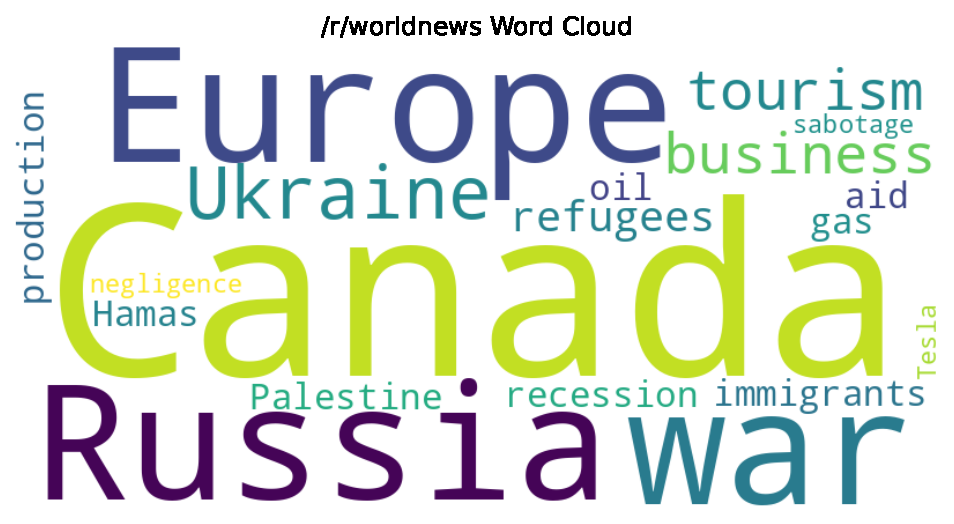
\includegraphics[keepaspectratio]{detecting_bots_on_reddit_code_files/figure-pdf/cell-29-output-3.pdf}}

\subcaption{\label{}r/worldnews}
\end{minipage}%
%
\begin{minipage}{0.50\linewidth}

\pandocbounded{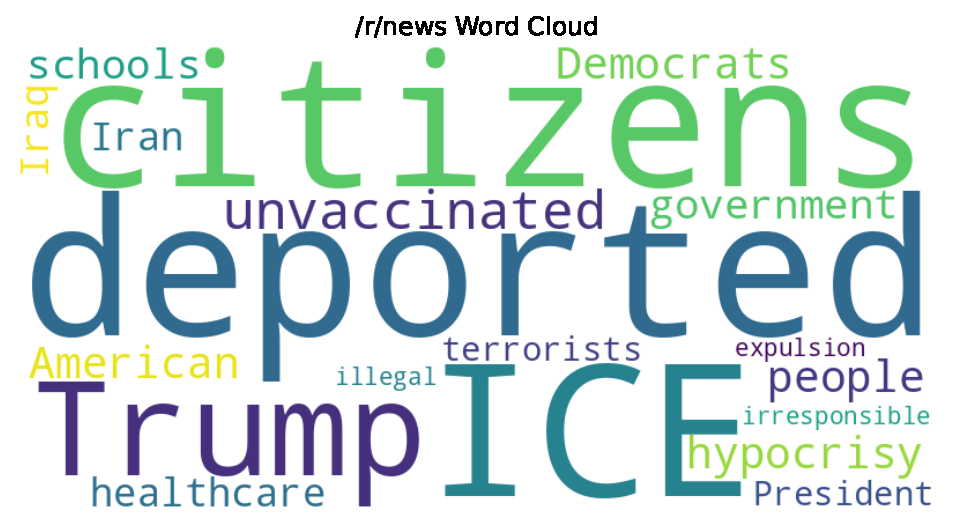
\includegraphics[keepaspectratio]{detecting_bots_on_reddit_code_files/figure-pdf/cell-29-output-4.pdf}}

\subcaption{\label{}r/news}
\end{minipage}%
\newline
\begin{minipage}{0.50\linewidth}

\pandocbounded{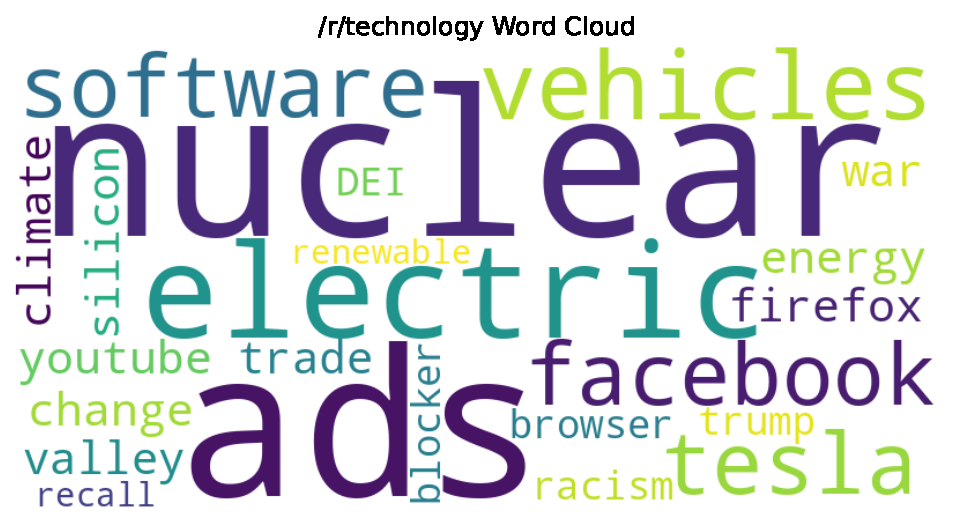
\includegraphics[keepaspectratio]{detecting_bots_on_reddit_code_files/figure-pdf/cell-29-output-5.pdf}}

\subcaption{\label{}r/technology}
\end{minipage}%
%
\begin{minipage}{0.50\linewidth}

\pandocbounded{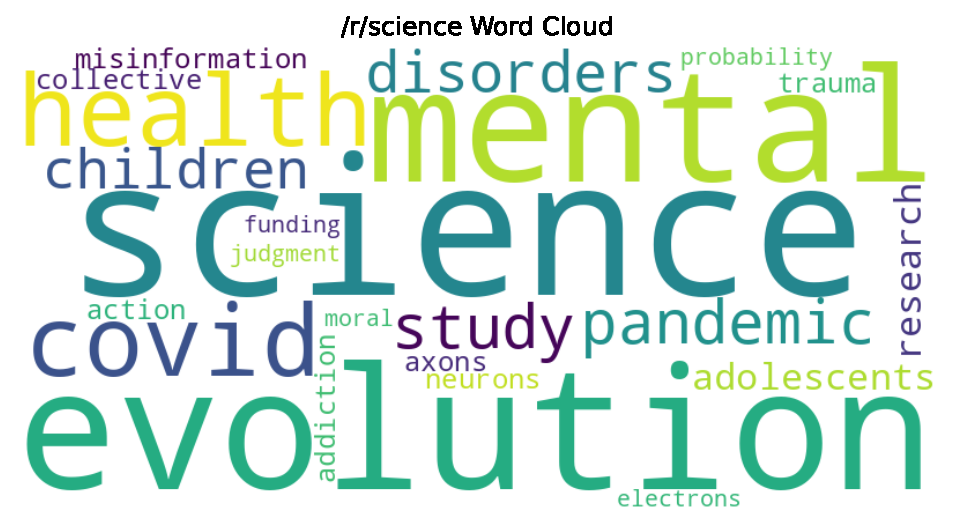
\includegraphics[keepaspectratio]{detecting_bots_on_reddit_code_files/figure-pdf/cell-29-output-6.pdf}}

\subcaption{\label{}r/science}
\end{minipage}%

\caption{\label{fig-wordclouds-gemini}Word Clouds generated by Gemini
for the 4 subreddits that were not shown in the main document body.}

\end{figure}%

\begin{figure}

\begin{minipage}{0.33\linewidth}

\pandocbounded{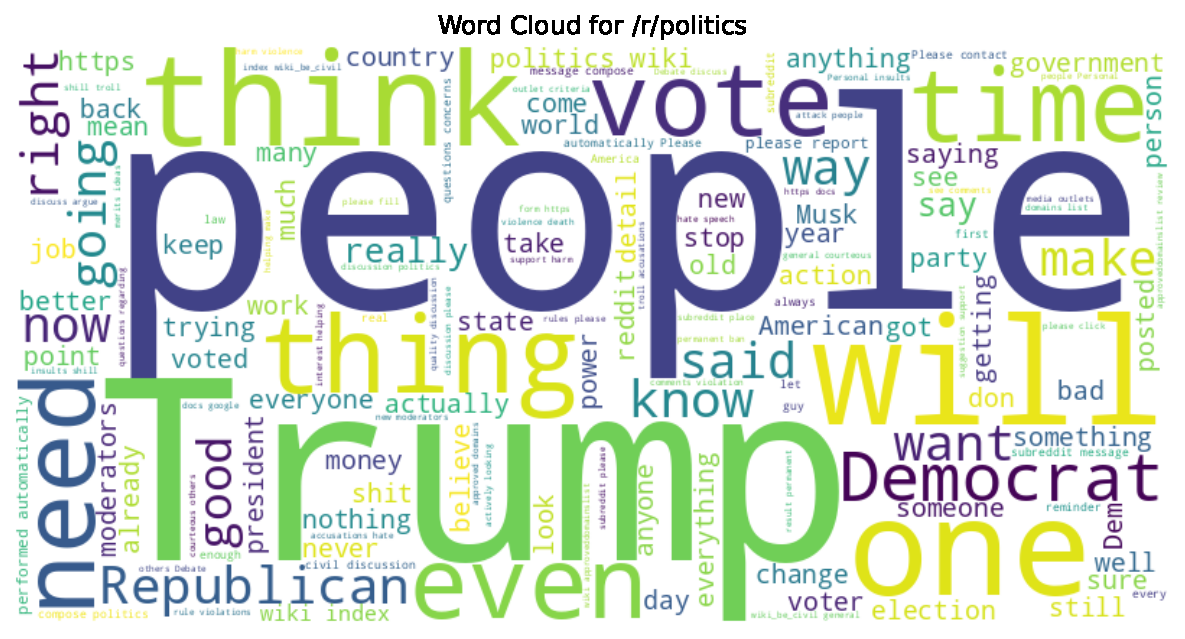
\includegraphics[keepaspectratio]{detecting_bots_on_reddit_code_files/figure-pdf/cell-27-output-3.pdf}}

\subcaption{\label{}r/politics}
\end{minipage}%
%
\begin{minipage}{0.33\linewidth}

\pandocbounded{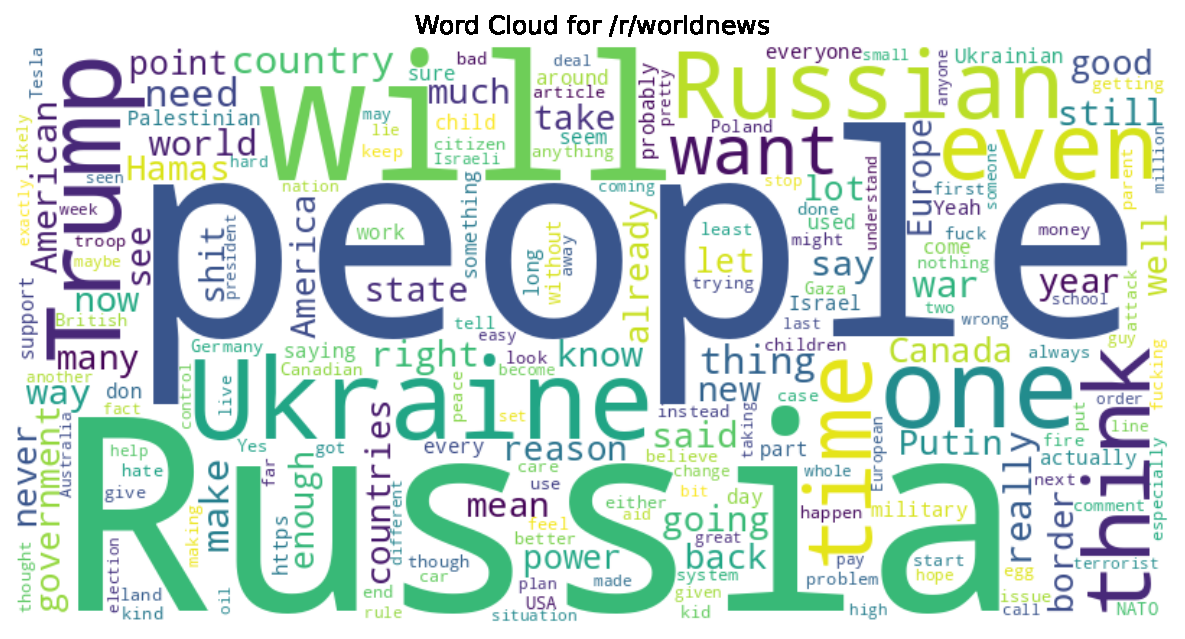
\includegraphics[keepaspectratio]{detecting_bots_on_reddit_code_files/figure-pdf/cell-27-output-6.pdf}}

\subcaption{\label{}r/worldnews}
\end{minipage}%
%
\begin{minipage}{0.33\linewidth}

\pandocbounded{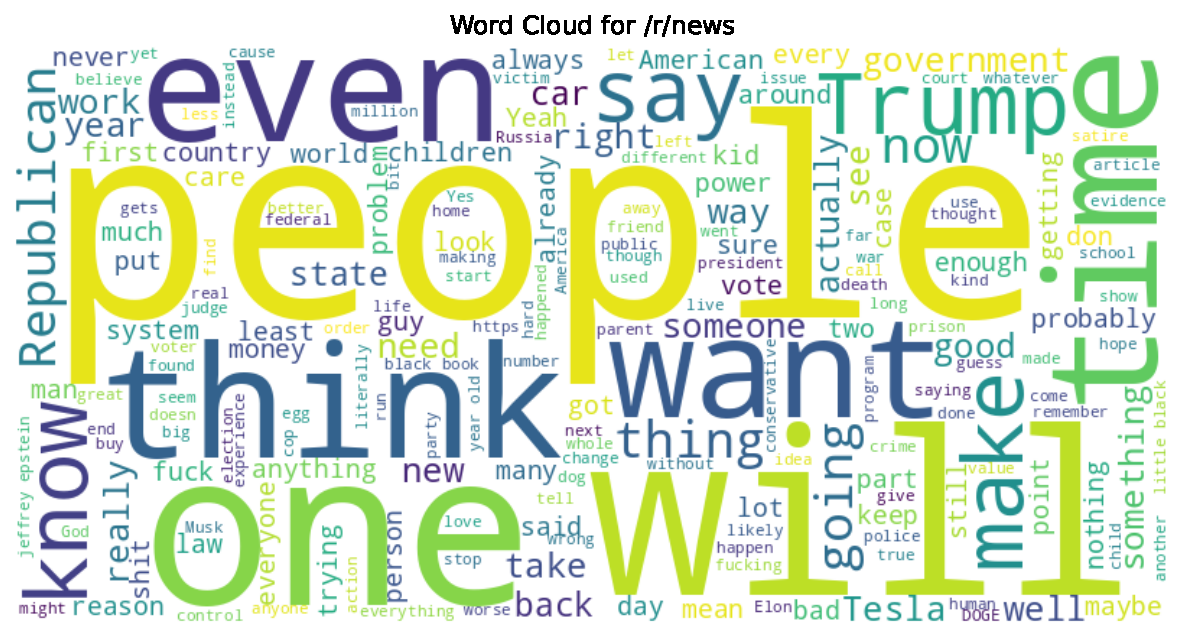
\includegraphics[keepaspectratio]{detecting_bots_on_reddit_code_files/figure-pdf/cell-27-output-2.pdf}}

\subcaption{\label{}r/news}
\end{minipage}%
\newline
\begin{minipage}{0.33\linewidth}

\pandocbounded{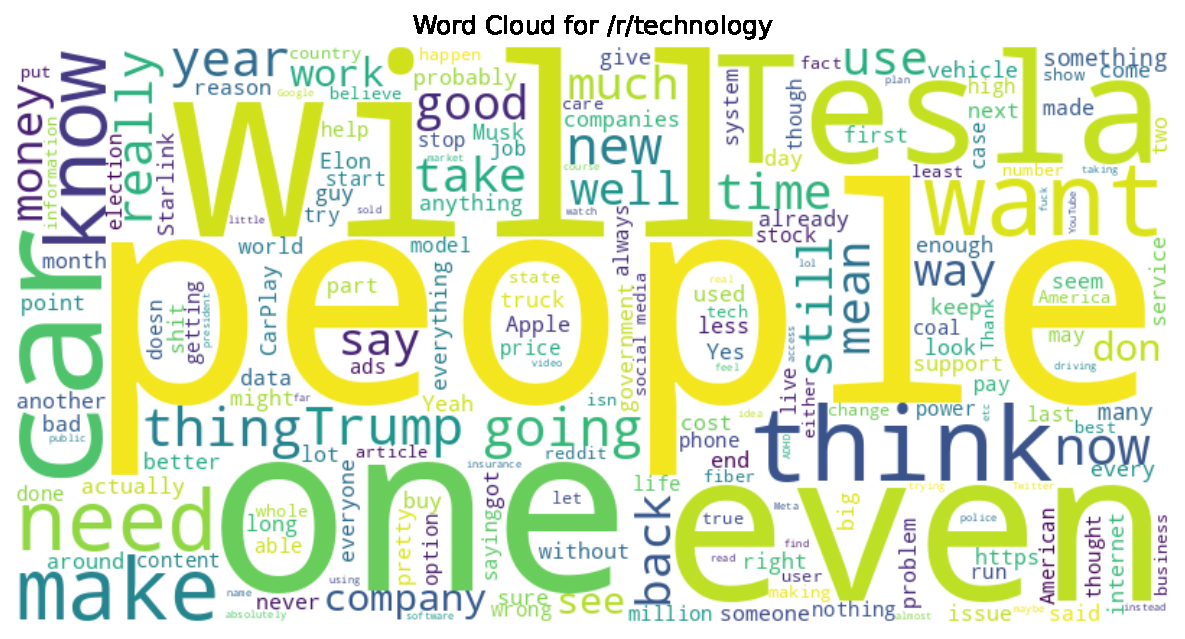
\includegraphics[keepaspectratio]{detecting_bots_on_reddit_code_files/figure-pdf/cell-27-output-5.pdf}}

\subcaption{\label{}r/technology}
\end{minipage}%
%
\begin{minipage}{0.33\linewidth}

\pandocbounded{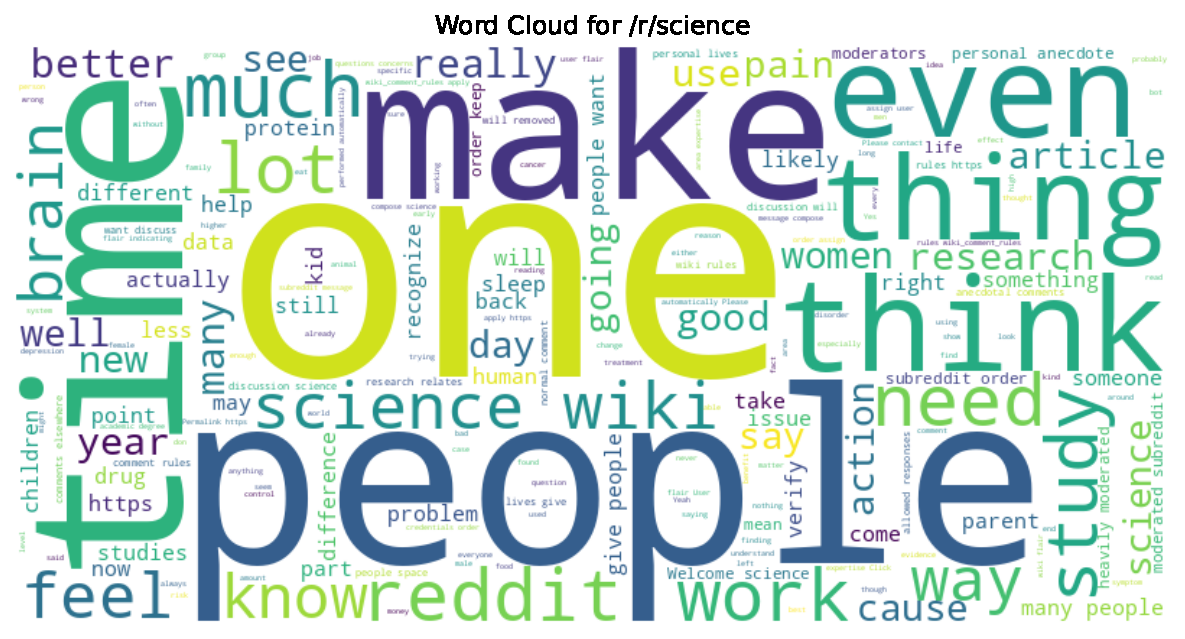
\includegraphics[keepaspectratio]{detecting_bots_on_reddit_code_files/figure-pdf/cell-27-output-4.pdf}}

\subcaption{\label{}r/science}
\end{minipage}%

\caption{\label{fig-wordclouds-freq}Word Clouds generated by simply
looking at word frequency for all 5 subreddits. You can notice that some
words which do not appear specific to any one subreddit are more
commonly shown here, informing the need for either a more sophisticated
method of creating the word cloud, or simply the adoption of LLMs for
Word Cloud generation.}

\end{figure}%

\begin{figure}[H]

{\centering \pandocbounded{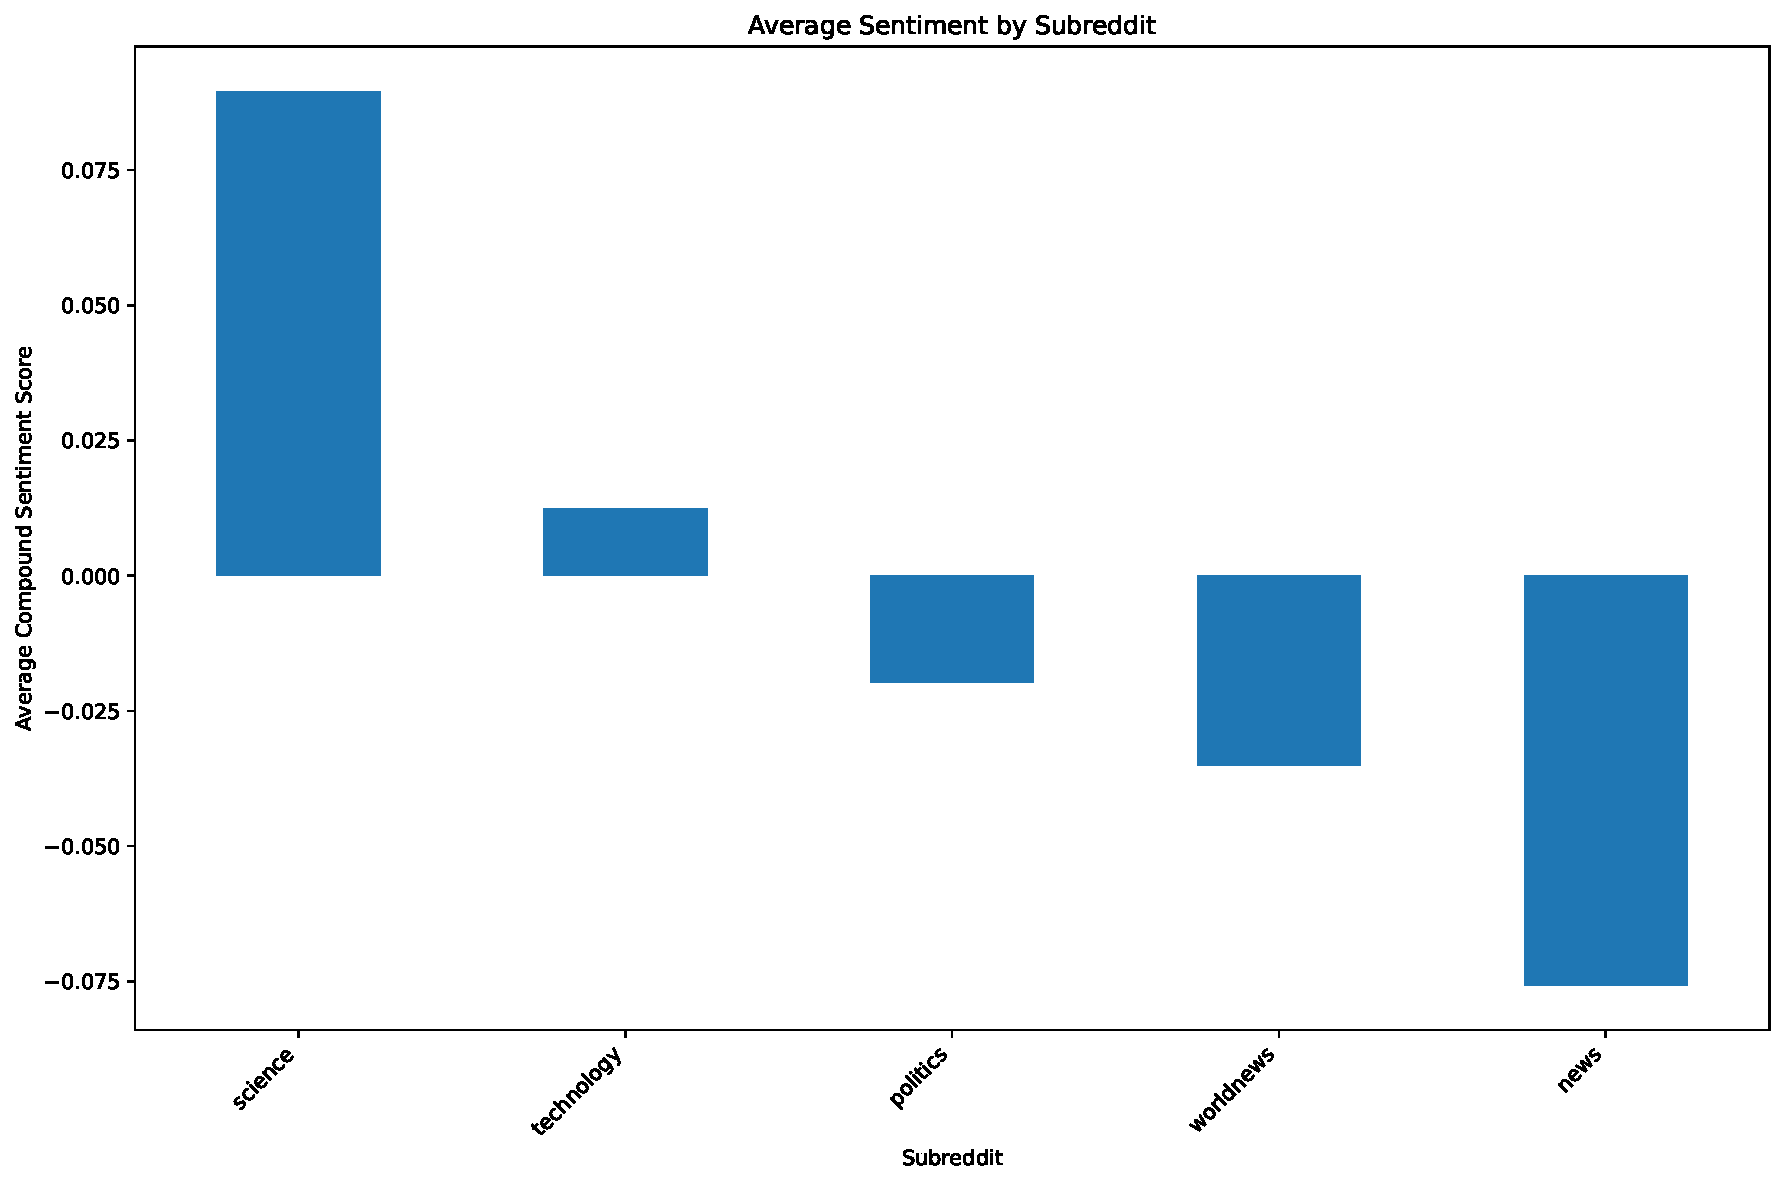
\includegraphics[keepaspectratio]{detecting_bots_on_reddit_code_files/figure-pdf/cell-27-output-1.pdf}}

}

\caption{Average Compound Sentiment Scores by subreddit. Higher score
indicates a more positive sentiment.}

\end{figure}%%
\begin{figure}[H]

{\centering \pandocbounded{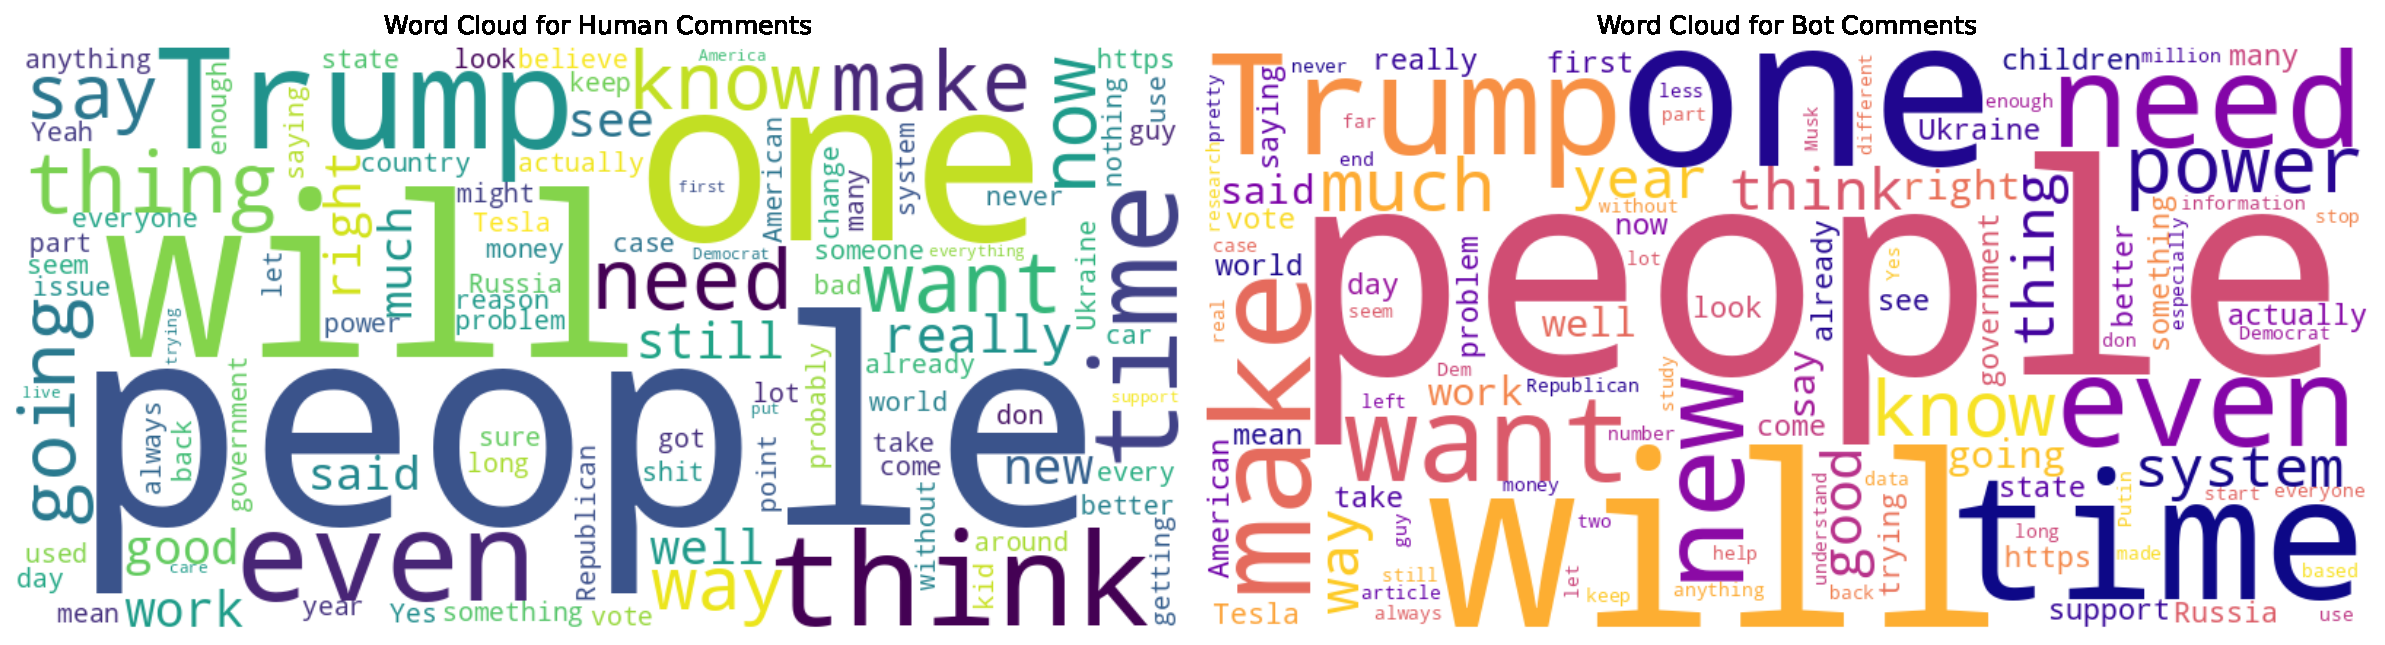
\includegraphics[keepaspectratio]{detecting_bots_on_reddit_code_files/figure-pdf/cell-25-output-2.pdf}}

}

\caption{Word Clouds (generated by simple text frequency analysis)
showing that users and bots do not have significantly different term
usage patterns.}

\end{figure}%%
\begin{figure}[H]

{\centering \pandocbounded{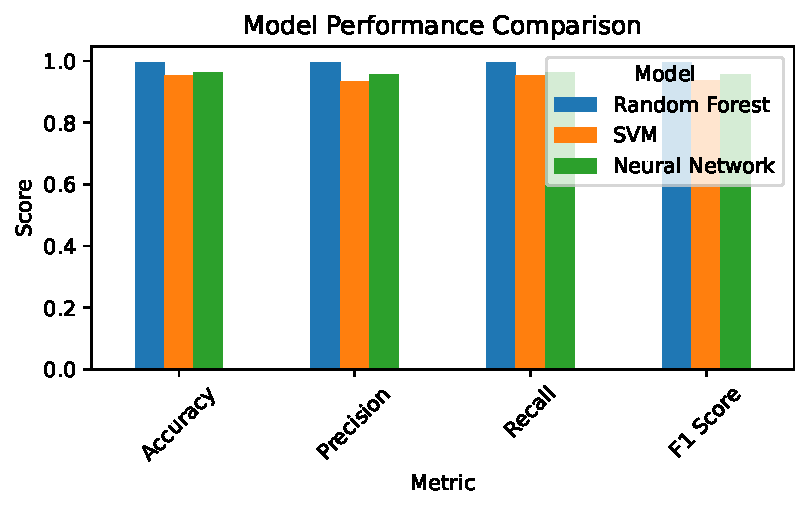
\includegraphics[keepaspectratio]{detecting_bots_on_reddit_code_files/figure-pdf/cell-22-output-4.pdf}}

}

\caption{Performance of each of the 3 models in predicting heuristically
labeled user class on a simple train/test split.}

\end{figure}%




\end{document}
